\documentclass[]{book}
\usepackage{lmodern}
\usepackage{amssymb,amsmath}
\usepackage{ifxetex,ifluatex}
\usepackage{fixltx2e} % provides \textsubscript
\ifnum 0\ifxetex 1\fi\ifluatex 1\fi=0 % if pdftex
  \usepackage[T1]{fontenc}
  \usepackage[utf8]{inputenc}
\else % if luatex or xelatex
  \ifxetex
    \usepackage{mathspec}
  \else
    \usepackage{fontspec}
  \fi
  \defaultfontfeatures{Ligatures=TeX,Scale=MatchLowercase}
\fi
% use upquote if available, for straight quotes in verbatim environments
\IfFileExists{upquote.sty}{\usepackage{upquote}}{}
% use microtype if available
\IfFileExists{microtype.sty}{%
\usepackage{microtype}
\UseMicrotypeSet[protrusion]{basicmath} % disable protrusion for tt fonts
}{}
\usepackage[margin=1in]{geometry}
\usepackage{hyperref}
\hypersetup{unicode=true,
            pdftitle={Statistics 1},
            pdfborder={0 0 0},
            breaklinks=true}
\urlstyle{same}  % don't use monospace font for urls
\usepackage{color}
\usepackage{fancyvrb}
\newcommand{\VerbBar}{|}
\newcommand{\VERB}{\Verb[commandchars=\\\{\}]}
\DefineVerbatimEnvironment{Highlighting}{Verbatim}{commandchars=\\\{\}}
% Add ',fontsize=\small' for more characters per line
\usepackage{framed}
\definecolor{shadecolor}{RGB}{248,248,248}
\newenvironment{Shaded}{\begin{snugshade}}{\end{snugshade}}
\newcommand{\KeywordTok}[1]{\textcolor[rgb]{0.13,0.29,0.53}{\textbf{#1}}}
\newcommand{\DataTypeTok}[1]{\textcolor[rgb]{0.13,0.29,0.53}{#1}}
\newcommand{\DecValTok}[1]{\textcolor[rgb]{0.00,0.00,0.81}{#1}}
\newcommand{\BaseNTok}[1]{\textcolor[rgb]{0.00,0.00,0.81}{#1}}
\newcommand{\FloatTok}[1]{\textcolor[rgb]{0.00,0.00,0.81}{#1}}
\newcommand{\ConstantTok}[1]{\textcolor[rgb]{0.00,0.00,0.00}{#1}}
\newcommand{\CharTok}[1]{\textcolor[rgb]{0.31,0.60,0.02}{#1}}
\newcommand{\SpecialCharTok}[1]{\textcolor[rgb]{0.00,0.00,0.00}{#1}}
\newcommand{\StringTok}[1]{\textcolor[rgb]{0.31,0.60,0.02}{#1}}
\newcommand{\VerbatimStringTok}[1]{\textcolor[rgb]{0.31,0.60,0.02}{#1}}
\newcommand{\SpecialStringTok}[1]{\textcolor[rgb]{0.31,0.60,0.02}{#1}}
\newcommand{\ImportTok}[1]{#1}
\newcommand{\CommentTok}[1]{\textcolor[rgb]{0.56,0.35,0.01}{\textit{#1}}}
\newcommand{\DocumentationTok}[1]{\textcolor[rgb]{0.56,0.35,0.01}{\textbf{\textit{#1}}}}
\newcommand{\AnnotationTok}[1]{\textcolor[rgb]{0.56,0.35,0.01}{\textbf{\textit{#1}}}}
\newcommand{\CommentVarTok}[1]{\textcolor[rgb]{0.56,0.35,0.01}{\textbf{\textit{#1}}}}
\newcommand{\OtherTok}[1]{\textcolor[rgb]{0.56,0.35,0.01}{#1}}
\newcommand{\FunctionTok}[1]{\textcolor[rgb]{0.00,0.00,0.00}{#1}}
\newcommand{\VariableTok}[1]{\textcolor[rgb]{0.00,0.00,0.00}{#1}}
\newcommand{\ControlFlowTok}[1]{\textcolor[rgb]{0.13,0.29,0.53}{\textbf{#1}}}
\newcommand{\OperatorTok}[1]{\textcolor[rgb]{0.81,0.36,0.00}{\textbf{#1}}}
\newcommand{\BuiltInTok}[1]{#1}
\newcommand{\ExtensionTok}[1]{#1}
\newcommand{\PreprocessorTok}[1]{\textcolor[rgb]{0.56,0.35,0.01}{\textit{#1}}}
\newcommand{\AttributeTok}[1]{\textcolor[rgb]{0.77,0.63,0.00}{#1}}
\newcommand{\RegionMarkerTok}[1]{#1}
\newcommand{\InformationTok}[1]{\textcolor[rgb]{0.56,0.35,0.01}{\textbf{\textit{#1}}}}
\newcommand{\WarningTok}[1]{\textcolor[rgb]{0.56,0.35,0.01}{\textbf{\textit{#1}}}}
\newcommand{\AlertTok}[1]{\textcolor[rgb]{0.94,0.16,0.16}{#1}}
\newcommand{\ErrorTok}[1]{\textcolor[rgb]{0.64,0.00,0.00}{\textbf{#1}}}
\newcommand{\NormalTok}[1]{#1}
\usepackage{longtable,booktabs}
\usepackage{graphicx,grffile}
\makeatletter
\def\maxwidth{\ifdim\Gin@nat@width>\linewidth\linewidth\else\Gin@nat@width\fi}
\def\maxheight{\ifdim\Gin@nat@height>\textheight\textheight\else\Gin@nat@height\fi}
\makeatother
% Scale images if necessary, so that they will not overflow the page
% margins by default, and it is still possible to overwrite the defaults
% using explicit options in \includegraphics[width, height, ...]{}
\setkeys{Gin}{width=\maxwidth,height=\maxheight,keepaspectratio}
\IfFileExists{parskip.sty}{%
\usepackage{parskip}
}{% else
\setlength{\parindent}{0pt}
\setlength{\parskip}{6pt plus 2pt minus 1pt}
}
\setlength{\emergencystretch}{3em}  % prevent overfull lines
\providecommand{\tightlist}{%
  \setlength{\itemsep}{0pt}\setlength{\parskip}{0pt}}
\setcounter{secnumdepth}{5}
% Redefines (sub)paragraphs to behave more like sections
\ifx\paragraph\undefined\else
\let\oldparagraph\paragraph
\renewcommand{\paragraph}[1]{\oldparagraph{#1}\mbox{}}
\fi
\ifx\subparagraph\undefined\else
\let\oldsubparagraph\subparagraph
\renewcommand{\subparagraph}[1]{\oldsubparagraph{#1}\mbox{}}
\fi

%%% Use protect on footnotes to avoid problems with footnotes in titles
\let\rmarkdownfootnote\footnote%
\def\footnote{\protect\rmarkdownfootnote}

%%% Change title format to be more compact
\usepackage{titling}

% Create subtitle command for use in maketitle
\newcommand{\subtitle}[1]{
  \posttitle{
    \begin{center}\large#1\end{center}
    }
}

\setlength{\droptitle}{-2em}
  \title{Statistics 1}
  \pretitle{\vspace{\droptitle}\centering\huge}
  \posttitle{\par}
  \author{}
  \preauthor{}\postauthor{}
  \date{}
  \predate{}\postdate{}


\usepackage{amsthm}
\newtheorem{theorem}{Theorem}[chapter]
\newtheorem{lemma}{Lemma}[chapter]
\theoremstyle{definition}
\newtheorem{definition}{Definition}[chapter]
\newtheorem{corollary}{Corollary}[chapter]
\newtheorem{proposition}{Proposition}[chapter]
\theoremstyle{definition}
\newtheorem{example}{Example}[chapter]
\theoremstyle{definition}
\newtheorem{exercise}{Exercise}[chapter]
\theoremstyle{remark}
\newtheorem*{remark}{Remark}
\newtheorem*{solution}{Solution}
\begin{document}
\maketitle

{
\setcounter{tocdepth}{1}
\tableofcontents
}
\chapter*{About this course}\label{about-this-course}
\addcontentsline{toc}{chapter}{About this course}

This course is an introduction to data science. We have three primary
aims. First, to introduce you to the logic of quantitative research
design. Second, to familiarise you with statistical models that
scientists and policy-makers use to answer social science questions.
Third, to help you acquire the necessary skills to conduct your own
quantitative research projects. No prior statistical knowledge is
assumed. We will use the statistical software R and RStudio on top.

\begin{center}\rule{0.5\linewidth}{\linethickness}\end{center}

Syllabus

Moodle

Piazza

\chapter{Introduction: Measurement, Central Tendency, Dispersion,
Validity,
Reliability}\label{introduction-measurement-central-tendency-dispersion-validity-reliability}

\section{Seminar}\label{seminar}

In this seminar session, we introduce working with R. We illustrate some
basic functionality and help you familiarise yourself with the look and
feel of RStudio. Measures of central tendency and dispersion are easy to
calculate in R. We focus on introducing the logic of R first and then
describe how central tendency and dispersion are calculated in the end
of the seminar.

\subsection{Getting Started}\label{getting-started}

Install R and RStudio on your computer by downloading them from the
following sources:

\begin{itemize}
\tightlist
\item
  Download R from \href{https://cran.r-project.org}{The Comprehensive R
  Archive Network (CRAN)}
\item
  Download RStudio from \href{https://www.rstudio.com}{RStudio.com}
\end{itemize}

\subsection{RStudio}\label{rstudio}

Let's get acquainted with R. When you start RStudio for the first time,
you'll see three panes:

\begin{figure}
\centering
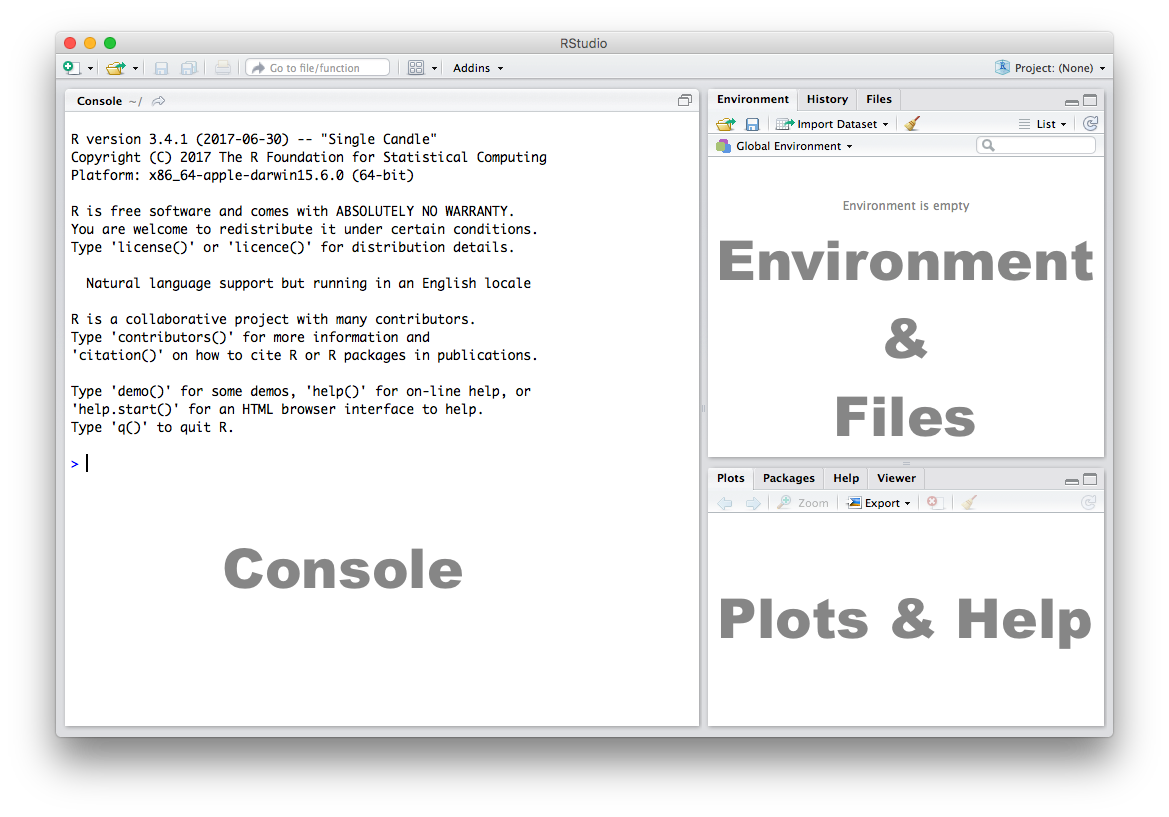
\includegraphics{./img/rstudio_default.png}
\caption{}
\end{figure}

\subsection{Console}\label{console}

The Console in RStudio is the simplest way to interact with R. You can
type some code at the Console and when you press ENTER, R will run that
code. Depending on what you type, you may see some output in the Console
or if you make a mistake, you may get a warning or an error message.

Let's familiarize ourselves with the console by using R as a simple
calculator:

\begin{Shaded}
\begin{Highlighting}[]
\DecValTok{2} \OperatorTok{+}\StringTok{ }\DecValTok{4}
\end{Highlighting}
\end{Shaded}

\begin{verbatim}
[1] 6
\end{verbatim}

Now that we know how to use the \texttt{+} sign for addition, let's try
some other mathematical operations such as subtraction (\texttt{-}),
multiplication (\texttt{*}), and division (\texttt{/}).

\begin{Shaded}
\begin{Highlighting}[]
\DecValTok{10} \OperatorTok{-}\StringTok{ }\DecValTok{4}
\end{Highlighting}
\end{Shaded}

\begin{verbatim}
[1] 6
\end{verbatim}

\begin{Shaded}
\begin{Highlighting}[]
\DecValTok{5} \OperatorTok{*}\StringTok{ }\DecValTok{3}
\end{Highlighting}
\end{Shaded}

\begin{verbatim}
[1] 15
\end{verbatim}

\begin{Shaded}
\begin{Highlighting}[]
\DecValTok{7} \OperatorTok{/}\StringTok{ }\DecValTok{2}
\end{Highlighting}
\end{Shaded}

\begin{verbatim}
[1] 3.5
\end{verbatim}

\begin{longtable}[]{@{}ll@{}}
\toprule
\begin{minipage}[t]{0.69\columnwidth}\raggedright\strut
You can use the cursor or arrow keys on your keyboard to edit your code
at the console:- Use the UP and DOWN keys to re-run something without
typing it again- Use the LEFT and RIGHT keys to edit\strut
\end{minipage} & \begin{minipage}[t]{0.25\columnwidth}\raggedright\strut
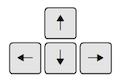
\includegraphics{./img/rstudio_cursorkeys.png}\strut
\end{minipage}\tabularnewline
\bottomrule
\end{longtable}

Take a few minutes to play around at the console and try different
things out. Don't worry if you make a mistake, you can't break anything
easily!

\subsection{Functions}\label{functions}

Functions are a set of instructions that carry out a specific task.
Functions often require some input and generate some output. For
example, instead of using the \texttt{+} operator for addition, we can
use the \texttt{sum} function to add two or more numbers.

\begin{Shaded}
\begin{Highlighting}[]
\KeywordTok{sum}\NormalTok{(}\DecValTok{1}\NormalTok{, }\DecValTok{4}\NormalTok{, }\DecValTok{10}\NormalTok{)}
\end{Highlighting}
\end{Shaded}

\begin{verbatim}
[1] 15
\end{verbatim}

In the example above, \texttt{1,\ 4,\ 10} are the inputs and 15 is the
output. A function always requires the use of parenthesis or round
brackets \texttt{()}. Inputs to the function are called
\textbf{arguments} and go inside the brackets. The output of a function
is displayed on the screen but we can also have the option of saving the
result of the output. More on this later.

\subsection{Getting Help}\label{getting-help}

Another useful function in R is \texttt{help} which we can use to
display online documentation. For example, if we wanted to know how to
use the \texttt{sum} function, we could type \texttt{help(sum)} and look
at the online documentation.

\begin{Shaded}
\begin{Highlighting}[]
\KeywordTok{help}\NormalTok{(sum)}
\end{Highlighting}
\end{Shaded}

The question mark \texttt{?} can also be used as a shortcut to access
online help.

\begin{Shaded}
\begin{Highlighting}[]
\NormalTok{?sum}
\end{Highlighting}
\end{Shaded}

\begin{figure}
\centering
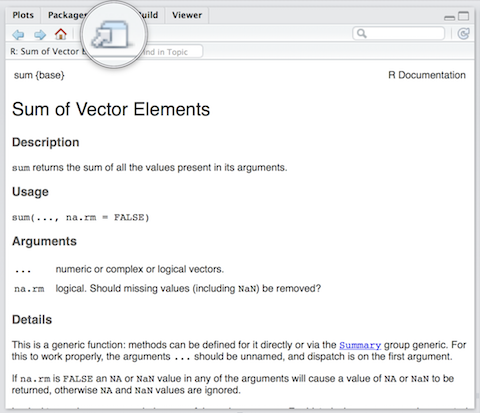
\includegraphics{./img/rstudio_help.png}
\caption{}
\end{figure}

Use the toolbar button shown in the picture above to expand and display
the help in a new window.

Help pages for functions in R follow a consistent layout generally
include these sections:

\begin{longtable}[]{@{}ll@{}}
\toprule
Description & A brief description of the function\tabularnewline
Usage & The complete syntax or grammar including all arguments
(inputs)\tabularnewline
Arguments & Explanation of each argument\tabularnewline
Details & Any relevant details about the function and its
arguments\tabularnewline
Value & The output value of the function\tabularnewline
Examples & Example of how to use the function\tabularnewline
\bottomrule
\end{longtable}

\subsection{The Assignment Operator}\label{the-assignment-operator}

Now we know how to provide inputs to a function using parenthesis or
round brackets \texttt{()}, but what about the output of a function?

We use the assignment operator \textbf{\texttt{\textless{}-}} for
creating or updating objects. If we wanted to save the result of adding
\texttt{sum(1,\ 4,\ 10)}, we would do the following:

\begin{Shaded}
\begin{Highlighting}[]
\NormalTok{myresult <-}\StringTok{ }\KeywordTok{sum}\NormalTok{(}\DecValTok{1}\NormalTok{, }\DecValTok{4}\NormalTok{, }\DecValTok{10}\NormalTok{)}
\end{Highlighting}
\end{Shaded}

The line above creates a new object called \texttt{myresult} in our
environment and saves the result of the \texttt{sum(1,\ 4,\ 10)} in it.
To see what's in \texttt{myresult}, just type it at the console:

\begin{Shaded}
\begin{Highlighting}[]
\NormalTok{myresult}
\end{Highlighting}
\end{Shaded}

\begin{verbatim}
[1] 15
\end{verbatim}

Take a look at the \textbf{Environment} pane in RStudio and you'll see
\texttt{myresult} there.

\begin{figure}
\centering
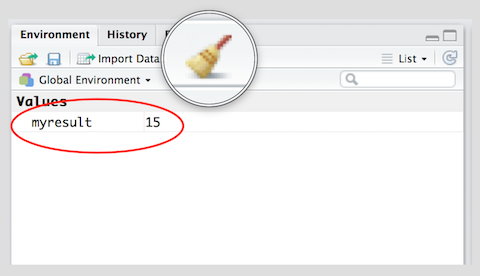
\includegraphics{./img/rstudio_env.png}
\caption{}
\end{figure}

To delete all objects from the environment, you can use the
\textbf{broom} button as shown in the picture above.

We called our object \texttt{myresult} but we can call it anything as
long as we follow a few simple rules. Object names can contain upper or
lower case letters (\texttt{A-Z}, \texttt{a-z}), numbers (\texttt{0-9}),
underscores (\texttt{\_}) or a dot (\texttt{.}) but all object names
must start with a letter. Choose names that are descriptive and easy to
type.

\begin{longtable}[]{@{}ll@{}}
\toprule
Good Object Names & Bad Object Names\tabularnewline
\midrule
\endhead
result & a\tabularnewline
myresult & x1\tabularnewline
my.result & this.name.is.just.too.long\tabularnewline
my\_result &\tabularnewline
data1 &\tabularnewline
\bottomrule
\end{longtable}

\subsection{Sequences}\label{sequences}

We often need to create sequences when manipulating data. For instance,
you might want to perform an operation on the first 10 rows of a dataset
so we need a way to select the range we're interested in.

There are two ways to create a sequence. Let's try to create a sequence
of numbers from 1 to 10 using the two methods:

\begin{enumerate}
\def\labelenumi{\arabic{enumi}.}
\tightlist
\item
  Using the colon \texttt{:} operator. If you're familiar with
  spreadsheets then you might've already used \texttt{:} to select
  cells, for example \texttt{A1:A20}. In R, you can use the \texttt{:}
  to create a sequence in a similar fashion:
\end{enumerate}

\begin{Shaded}
\begin{Highlighting}[]
\DecValTok{1}\OperatorTok{:}\DecValTok{10}
\end{Highlighting}
\end{Shaded}

\begin{verbatim}
 [1]  1  2  3  4  5  6  7  8  9 10
\end{verbatim}

\begin{enumerate}
\def\labelenumi{\arabic{enumi}.}
\tightlist
\item
  Using the \texttt{seq} function we get the exact same result:
\end{enumerate}

\begin{Shaded}
\begin{Highlighting}[]
\KeywordTok{seq}\NormalTok{(}\DataTypeTok{from =} \DecValTok{1}\NormalTok{, }\DataTypeTok{to =} \DecValTok{10}\NormalTok{)}
\end{Highlighting}
\end{Shaded}

\begin{verbatim}
 [1]  1  2  3  4  5  6  7  8  9 10
\end{verbatim}

The \texttt{seq} function has a number of options which control how the
sequence is generated. For example to create a sequence from 0 to 100 in
increments of \texttt{5}, we can use the optional \texttt{by} argument.
Notice how we wrote \texttt{by\ =\ 5} as the third argument. It is a
common practice to specify the name of argument when the argument is
optional. The arguments \texttt{from} and \texttt{to} are not optional,
se we can write \texttt{seq(0,\ 100,\ by\ =\ 5)} instead of
\texttt{seq(from\ =\ 0,\ to\ =\ 100,\ by\ =\ 5)}. Both, are valid ways
of achieving the same outcome. You can code whichever way you like. We
recommend to write code such that you make it easy for your future self
and others to read and understand the code.

\begin{Shaded}
\begin{Highlighting}[]
\KeywordTok{seq}\NormalTok{(}\DataTypeTok{from =} \DecValTok{0}\NormalTok{, }\DataTypeTok{to =} \DecValTok{100}\NormalTok{, }\DataTypeTok{by =} \DecValTok{5}\NormalTok{)}
\end{Highlighting}
\end{Shaded}

\begin{verbatim}
 [1]   0   5  10  15  20  25  30  35  40  45  50  55  60  65  70  75  80
[18]  85  90  95 100
\end{verbatim}

Another common use of the \texttt{seq} function is to create a sequence
of a specific length. Here, we create a sequence from 0 to 100 with
length 9, i.e., the result is a vector with 9 elements.

\begin{Shaded}
\begin{Highlighting}[]
\KeywordTok{seq}\NormalTok{(}\DataTypeTok{from =} \DecValTok{0}\NormalTok{, }\DataTypeTok{to =} \DecValTok{100}\NormalTok{, }\DataTypeTok{length.out =}  \DecValTok{9}\NormalTok{)}
\end{Highlighting}
\end{Shaded}

\begin{verbatim}
[1]   0.0  12.5  25.0  37.5  50.0  62.5  75.0  87.5 100.0
\end{verbatim}

Now it's your turn:

\begin{itemize}
\tightlist
\item
  Create a sequence of \textbf{odd} numbers between 0 and 100 and save
  it in an object called \texttt{odd\_numbers}
\end{itemize}

\begin{Shaded}
\begin{Highlighting}[]
\NormalTok{odd_numbers <-}\StringTok{ }\KeywordTok{seq}\NormalTok{(}\DecValTok{1}\NormalTok{, }\DecValTok{100}\NormalTok{, }\DecValTok{2}\NormalTok{)}
\end{Highlighting}
\end{Shaded}

\begin{itemize}
\tightlist
\item
  Next, display \texttt{odd\_numbers} on the console to verify that you
  did it correctly
\end{itemize}

\begin{Shaded}
\begin{Highlighting}[]
\NormalTok{odd_numbers}
\end{Highlighting}
\end{Shaded}

\begin{verbatim}
 [1]  1  3  5  7  9 11 13 15 17 19 21 23 25 27 29 31 33 35 37 39 41 43 45
[24] 47 49 51 53 55 57 59 61 63 65 67 69 71 73 75 77 79 81 83 85 87 89 91
[47] 93 95 97 99
\end{verbatim}

\begin{itemize}
\item
  What do the numbers in square brackets \texttt{{[}\ {]}} mean? Look at
  the number of values displayed in each line to find out the answer.
\item
  Use the \texttt{length} function to find out how many values are in
  the object \texttt{odd\_numbers}.

  \begin{itemize}
  \tightlist
  \item
    HINT: Try \texttt{help(length)} and look at the examples section at
    the end of the help screen.
  \end{itemize}
\end{itemize}

\begin{Shaded}
\begin{Highlighting}[]
\KeywordTok{length}\NormalTok{(odd_numbers)}
\end{Highlighting}
\end{Shaded}

\begin{verbatim}
[1] 50
\end{verbatim}

\subsection{Scripts}\label{scripts}

The Console is great for simple tasks but if you're working on a project
you would mostly likely want to save your work in some sort of a
document or a file. Scripts in R are just plain text files that contain
R code. You can edit a script just like you would edit a file in any
word processing or note-taking application.

Create a new script using the menu or the toolbar button as shown below.

\begin{figure}
\centering
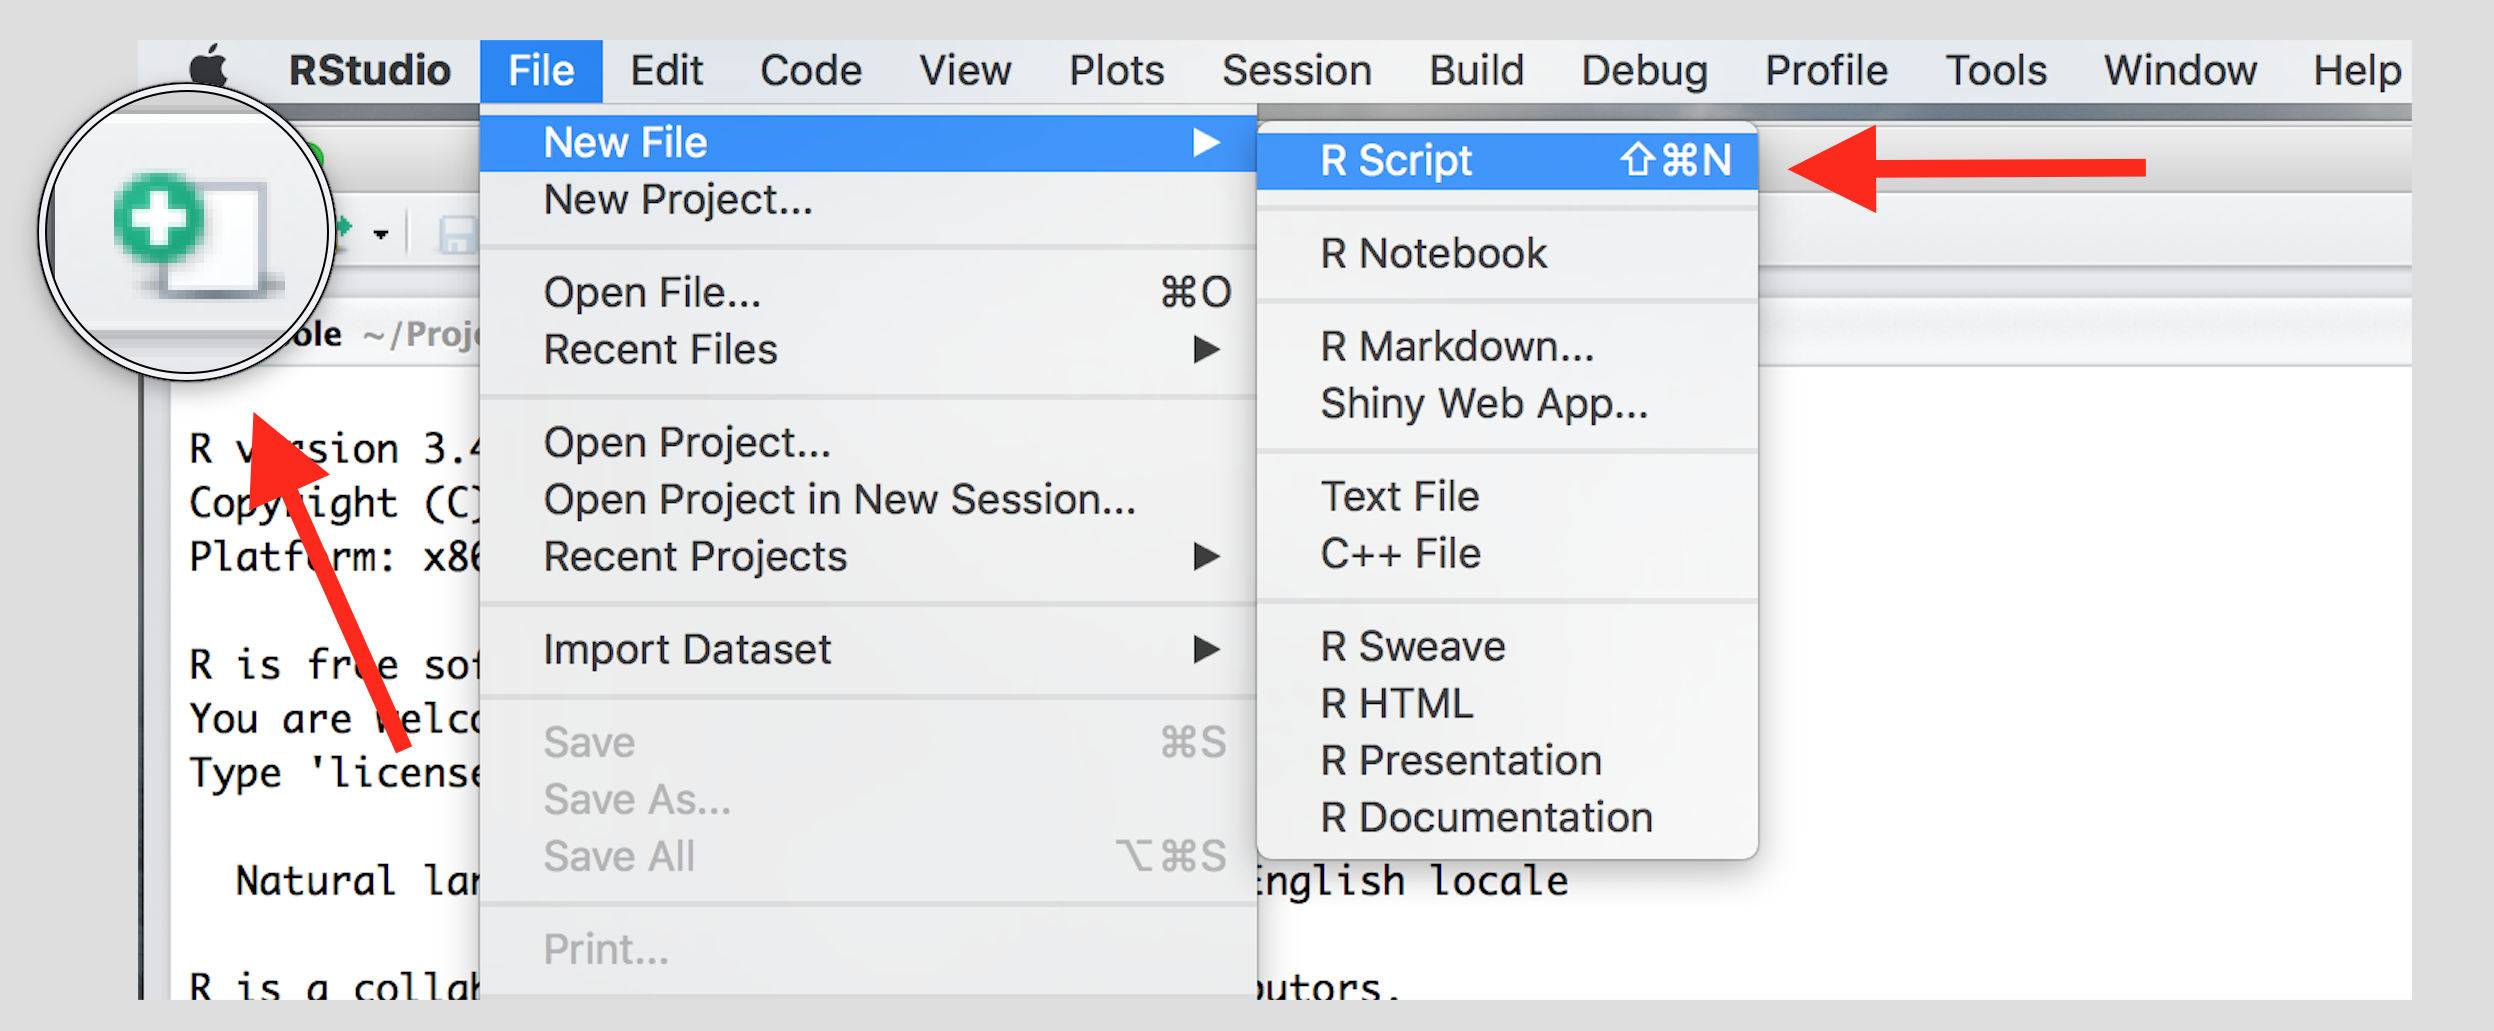
\includegraphics{./img/rstudio_newfile.png}
\caption{}
\end{figure}

Once you've created a script, it is generally a good idea to give it a
meaningful name and save it immediately. For our first session save your
script as \textbf{seminar1.R}

\begin{longtable}[]{@{}ll@{}}
\toprule
\begin{minipage}[t]{0.52\columnwidth}\raggedright\strut
Familiarize yourself with the script window in RStudio, and especially
the two buttons labeled \textbf{Run} and \textbf{Source}\strut
\end{minipage} & \begin{minipage}[t]{0.42\columnwidth}\raggedright\strut
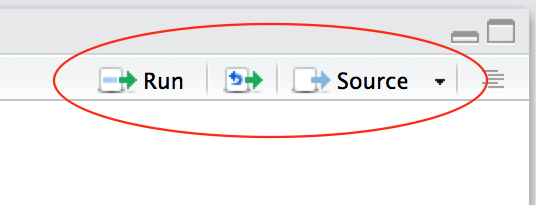
\includegraphics{./img/rstudio_script.png}\strut
\end{minipage}\tabularnewline
\bottomrule
\end{longtable}

There are a few different ways to run your code from a script.

\begin{longtable}[]{@{}ll@{}}
\toprule
\begin{minipage}[t]{0.24\columnwidth}\raggedright\strut
One line at a time\strut
\end{minipage} & \begin{minipage}[t]{0.70\columnwidth}\raggedright\strut
Place the cursor on the line you want to run and hit CTRL-ENTER or use
the \textbf{Run} button\strut
\end{minipage}\tabularnewline
\begin{minipage}[t]{0.24\columnwidth}\raggedright\strut
Multiple lines\strut
\end{minipage} & \begin{minipage}[t]{0.70\columnwidth}\raggedright\strut
Select the lines you want to run and hit CTRL-ENTER or use the
\textbf{Run} button\strut
\end{minipage}\tabularnewline
\begin{minipage}[t]{0.24\columnwidth}\raggedright\strut
Entire script\strut
\end{minipage} & \begin{minipage}[t]{0.70\columnwidth}\raggedright\strut
Use the \textbf{Source} button\strut
\end{minipage}\tabularnewline
\bottomrule
\end{longtable}

\subsection{Central Tendency}\label{central-tendency}

The appropriate measure of central tendency depends on the level of
measurement of the variable. To recap:

\begin{longtable}[]{@{}ll@{}}
\toprule
Level of measurement & Appropriate measure of central
tendency\tabularnewline
\midrule
\endhead
Continuous & arithmetic mean (or average)\tabularnewline
Ordered & median (or the central observation)\tabularnewline
Nominal & mode (the most frequent value)\tabularnewline
\bottomrule
\end{longtable}

\subsubsection{Mean}\label{mean}

We calculate the average grade on our eleven homework assignments in
statistics 1. We create our vector of 11 (fake) grades first using the
\texttt{c()} function, where \texttt{c} stands for collect or
concatenate.

\begin{Shaded}
\begin{Highlighting}[]
\NormalTok{hw.grades <-}\StringTok{ }\KeywordTok{c}\NormalTok{(}\DecValTok{80}\NormalTok{, }\DecValTok{90}\NormalTok{, }\DecValTok{85}\NormalTok{, }\DecValTok{71}\NormalTok{, }\DecValTok{69}\NormalTok{, }\DecValTok{85}\NormalTok{, }\DecValTok{83}\NormalTok{, }\DecValTok{88}\NormalTok{, }\DecValTok{99}\NormalTok{, }\DecValTok{81}\NormalTok{, }\DecValTok{92}\NormalTok{)}
\end{Highlighting}
\end{Shaded}

We now take the sum of the grades.

\begin{Shaded}
\begin{Highlighting}[]
\NormalTok{sum.hw.grades <-}\StringTok{ }\KeywordTok{sum}\NormalTok{(hw.grades)}
\end{Highlighting}
\end{Shaded}

We also take the number of grades

\begin{Shaded}
\begin{Highlighting}[]
\NormalTok{number.hw.grades <-}\StringTok{ }\KeywordTok{length}\NormalTok{(hw.grades) }
\end{Highlighting}
\end{Shaded}

The mean is the sum of grades over the number of grades.

\begin{Shaded}
\begin{Highlighting}[]
\NormalTok{sum.hw.grades }\OperatorTok{/}\StringTok{ }\NormalTok{number.hw.grades}
\end{Highlighting}
\end{Shaded}

\begin{verbatim}
[1] 83.90909
\end{verbatim}

R provides us with an even easier way to do the same with a function
called \href{http://bit.ly/R_mean}{\texttt{mean()}}.

\begin{Shaded}
\begin{Highlighting}[]
\KeywordTok{mean}\NormalTok{(hw.grades)}
\end{Highlighting}
\end{Shaded}

\begin{verbatim}
[1] 83.90909
\end{verbatim}

\subsubsection{Median}\label{median}

The median is the appropriate measure of central tendency for ordinal
variables. Ordinal means that there is a rank ordering but not equally
spaced intervals between values of the variable. Education is a common
example. In education, more education is better. But the difference
between primary school and secondary school is not the same as the
difference between secondary school and an undergraduate degree.

Let's generate a fake example with 100 people. We use numbers to code
different levels of education.

\begin{longtable}[]{@{}lll@{}}
\toprule
Code & Meaning & Frequency in our data\tabularnewline
0 & no education & 1\tabularnewline
1 & primary school & 5\tabularnewline
2 & secondary school & 55\tabularnewline
3 & undergraduate degree & 20\tabularnewline
4 & postgraduate degree & 10\tabularnewline
5 & doctorate & 9\tabularnewline
\bottomrule
\end{longtable}

We introduce a new function to create a vector. The function
\texttt{rep()}, replicates elements of a vector. Its arguments are the
item \texttt{x} to be replicated and the number of \texttt{times} to
replicate. Below, we create the variable education with the frequency of
education level indicated above. Note that the arguments \texttt{x} and
\texttt{times} do not have to be written out.

\begin{Shaded}
\begin{Highlighting}[]
\NormalTok{edu <-}\StringTok{ }\KeywordTok{c}\NormalTok{( }\KeywordTok{rep}\NormalTok{(}\DataTypeTok{x=}\DecValTok{0}\NormalTok{, }\DataTypeTok{times=}\DecValTok{1}\NormalTok{), }\KeywordTok{rep}\NormalTok{(}\DataTypeTok{x=}\DecValTok{1}\NormalTok{, }\DataTypeTok{times=}\DecValTok{5}\NormalTok{), }\KeywordTok{rep}\NormalTok{(}\DataTypeTok{x=}\DecValTok{2}\NormalTok{, }\DataTypeTok{times=}\DecValTok{55}\NormalTok{),}
          \KeywordTok{rep}\NormalTok{(}\DataTypeTok{x=}\DecValTok{3}\NormalTok{, }\DataTypeTok{times=}\DecValTok{20}\NormalTok{), }\KeywordTok{rep}\NormalTok{(}\DecValTok{4}\NormalTok{,}\DecValTok{10}\NormalTok{), }\KeywordTok{rep}\NormalTok{(}\DecValTok{5}\NormalTok{,}\DecValTok{9}\NormalTok{) )}
\end{Highlighting}
\end{Shaded}

The median level of education is the level where 50 percent of the
observations have a lower or equal level of education and 50 percent
have a higher or equal level of education. That means that the median
splits the data in half.

We use the \href{http://bit.ly/R_median}{\texttt{median()}} function for
finding the median.

\begin{Shaded}
\begin{Highlighting}[]
\KeywordTok{median}\NormalTok{(edu)}
\end{Highlighting}
\end{Shaded}

\begin{verbatim}
[1] 2
\end{verbatim}

The median level of education is secondary school.

\subsubsection{Mode}\label{mode}

The mode is the appropriate measure of central tendency if the level of
measurement is nominal. Nominal means that there is no ordering implicit
in the values that a variable takes on. We create data from 1000 (fake)
voters in the United Kingdom who each express their preference on
remaining in or leaving the European Union. The options are leave or
stay. Leaving is not greater than staying and vice versa (even though we
all order the two options normatively).

\begin{longtable}[]{@{}lll@{}}
\toprule
Code & Meaning & Frequency in our data\tabularnewline
0 & leave & 509\tabularnewline
1 & stay & 491\tabularnewline
\bottomrule
\end{longtable}

\begin{Shaded}
\begin{Highlighting}[]
\NormalTok{stay <-}\StringTok{ }\KeywordTok{c}\NormalTok{(}\KeywordTok{rep}\NormalTok{(}\DecValTok{0}\NormalTok{, }\DecValTok{509}\NormalTok{), }\KeywordTok{rep}\NormalTok{(}\DecValTok{1}\NormalTok{, }\DecValTok{491}\NormalTok{))}
\end{Highlighting}
\end{Shaded}

The mode is the most common value in the data. There is no mode function
in R. The most straightforward way to determine the mode is to use the
\href{http://bit.ly/R_table}{\texttt{table()}} function. It returns a
frequency table. We can easily see the mode in the table. As your coding
skills increase, you will see other ways of recovering the mode from a
vector.

\begin{Shaded}
\begin{Highlighting}[]
\KeywordTok{table}\NormalTok{(stay)}
\end{Highlighting}
\end{Shaded}

\begin{verbatim}
stay
  0   1 
509 491 
\end{verbatim}

The mode is leaving the EU because the number of `leavers' (0) is
greater than the number of `remainers' (1).

\subsection{Dispersion}\label{dispersion}

The appropriate measure of dispersion depends on the level of
measurement of the variable we wish to describe.

\begin{longtable}[]{@{}ll@{}}
\toprule
Level of measurement & Appropriate measure of dispersion\tabularnewline
\midrule
\endhead
Continuous & variance and/or standard deviation\tabularnewline
Ordered & range or interquartile range\tabularnewline
Nominal & proportion in each category\tabularnewline
\bottomrule
\end{longtable}

\subsubsection{Variance and standard
deviation}\label{variance-and-standard-deviation}

Both the variance and the standard deviation tell by how much an average
realisation of a variable differs from the mean of that variable. Let's
assume that our variable is income in the UK. Let's assume that its mean
is 35 000 per year. We also assume that the average deviation from 35
000 is 5 000. If we ask 100 people in the UK at random about their
income, we get 100 different answers. If we average the differences
betweeen the 100 answers and 35 000, we would get 5 000. Suppose that
the average income in France is also 35 000 per year but the average
deviation is 10 000 instead. This would imply that income is more
equally distributed in the UK than in France.

Dispersion is important to describe data as this example illustrates.
Although, mean income in our hypothetical example is the same in France
and the UK, the distribution is tighter in the UK. The figure below
illustrates our example:

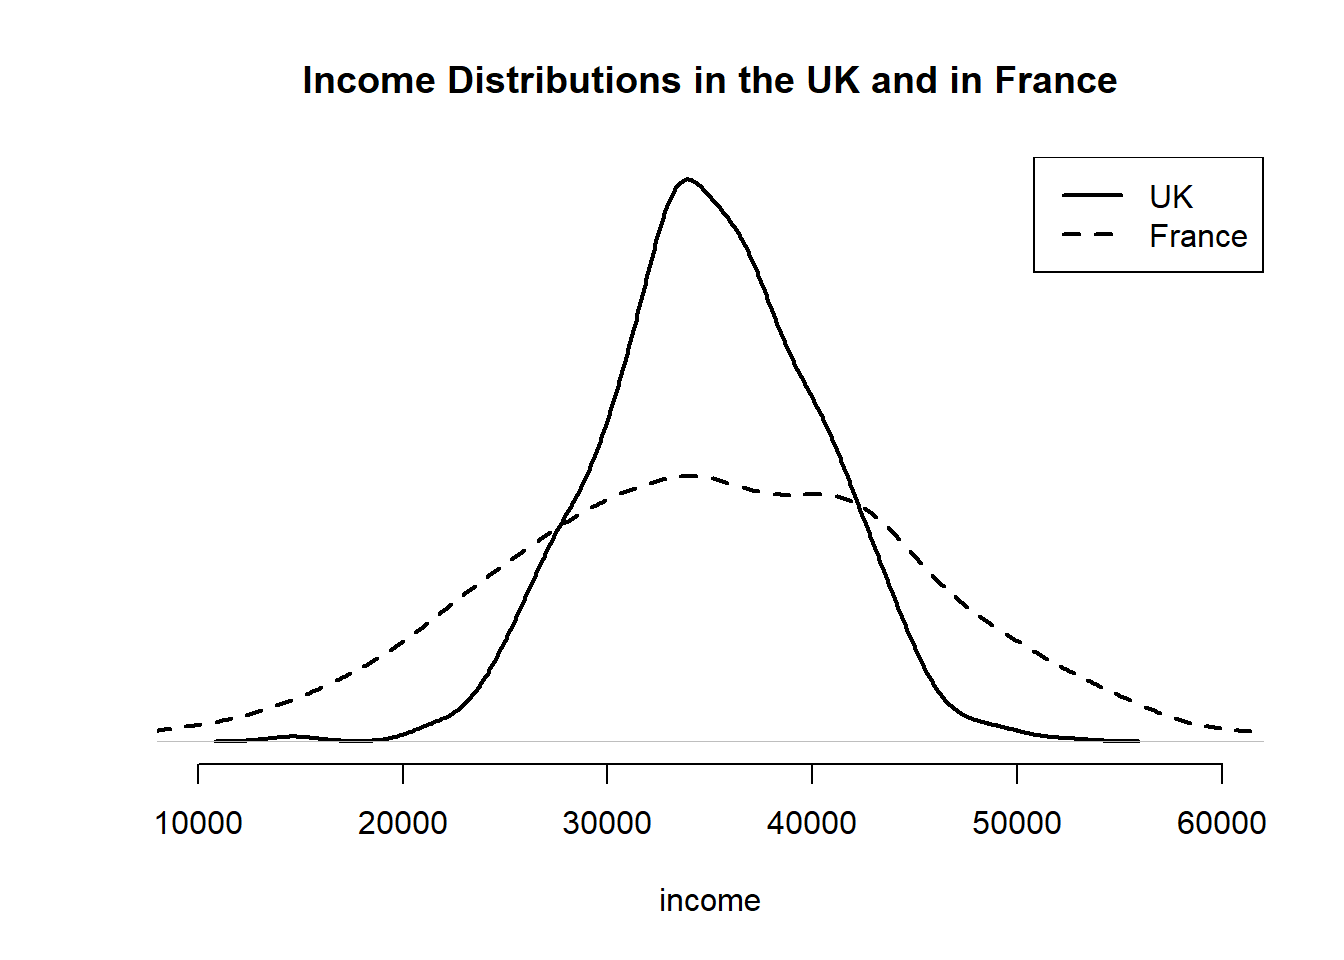
\includegraphics{statistics1_files/figure-latex/unnamed-chunk-26-1.pdf}

The variance gives us an idea about the variability of data. The formula
for the variance in the population is
\[ \frac{\sum_{i=1}^n(x_i - \mu_x)^2}{n}\]

The formula for the variance in a sample adjusts for sampling
variability, i.e., uncertainty about how well our sample reflects the
population by subtracting 1 in the denominator. Subtracting 1 will have
next to no effect if n is large but the effect increases the smaller n.
The smaller n, the larger the sample variance. The intuition is, that in
smaller samples, we are less certain that our sample reflects the
population. We, therefore, adjust variability of the data upwards. The
formula is

\[ \frac{\sum_{i=1}^n(x_i - \bar{x})^2}{n-1}\]

Notice the different notation for the mean in the two formulas. We write
\(\mu_x\) for the mean of x in the population and \(\bar{x}\) for the
mean of x in the sample. Notation is, however, unfortunately not always
consistent.

Take a minute to think your way through the formula. There are 4 setps:
(1), In the numerator, we subtract the mean of x from some realisation
of x. (2), We square the deviations from the mean because we want
positive numbers only. (3) We sum the squared deviations. (4) We divide
the sum by \((n-1)\). Below we show this for the homework example. In
the last row, we add a 5th step. We take the square root in order to
return to the orginial units of the homework grades.

\begin{longtable}[]{@{}llll@{}}
\toprule
Obs & Var & Dev. from mean & Squared dev. from mean\tabularnewline
\midrule
\endhead
i & grade & \(x_i-\bar{x}\) & \((x_i-\bar{x})^2\)\tabularnewline
1 & 80 & -3.9090909 & 15.2809917\tabularnewline
2 & 90 & 6.0909091 & 37.0991736\tabularnewline
3 & 85 & 1.0909091 & 1.1900826\tabularnewline
4 & 71 & -12.9090909 & 166.6446281\tabularnewline
5 & 69 & -14.9090909 & 222.2809917\tabularnewline
6 & 85 & 1.0909091 & 1.1900826\tabularnewline
7 & 83 & -0.9090909 & 0.8264463\tabularnewline
8 & 88 & 4.0909091 & 16.7355372\tabularnewline
9 & 99 & 15.0909091 & 227.7355372\tabularnewline
10 & 81 & -2.9090909 & 8.4628099\tabularnewline
11 & 92 & 8.0909091 & 65.4628099\tabularnewline
\(\sum_{i=1}^n\) & & & 762.9090909\tabularnewline
\(\div n-1\) & & & 76.2909091\tabularnewline
\(\sqrt{}\) & & & 8.7344667\tabularnewline
\bottomrule
\end{longtable}

Our first grade (80) is below the mean (83.9090909). The sum is, thus,
negative. Our second grade (90) is above the mean, so that the sum is
positive. Both are deviations from the mean (think of them as
distances). Our sum shall reflect the total sum of distances and
distances must be positive. Hence, we square the distances from the
mean. Having done this for all eleven observations, we sum the squared
distances. Dividing by 10 (with the sample adjustment), gives us the
average squared deviation. This is the variance. The units of the
variance---squared deviations---are somewhat awkward. We return to this
in a moment.

We take the variance in R by using the
\href{http://bit.ly/R_var}{\texttt{var()}} function. By default
\texttt{var()} takes the sample variance.

\begin{Shaded}
\begin{Highlighting}[]
\KeywordTok{var}\NormalTok{(hw.grades)}
\end{Highlighting}
\end{Shaded}

\begin{verbatim}
[1] 76.29091
\end{verbatim}

The average squared difference form our mean grade is 76.2909091. But
what does that mean? We would like to get rid of the square in our
units. That's what the standard deviation does. The standard deviation
is the square root over the variance.

\[ \sqrt{\frac{\sum_{i=1}^n(x_i - \bar{x})^2}{n-1}}\]

We get the average deviation from our mean grade (83.9090909) with the
\href{http://bit.ly/R_sd}{\texttt{sd()}} function.

\begin{Shaded}
\begin{Highlighting}[]
\KeywordTok{sd}\NormalTok{(hw.grades)}
\end{Highlighting}
\end{Shaded}

\begin{verbatim}
[1] 8.734467
\end{verbatim}

The standard deviation is much more intuitive than the variance because
its units are the same as the units of the variable we are interested
in. ``Why teach us about this awful variance then'', you ask.
Mathematically, we have to compute the variance before getting the
standard deviation. We recommend that you use the standard deviation to
describe the variability of your continuous data.

Note: We used the sample variance and sample standard deviation
formulas. If the eleven assignments represent the population, we would
use the population variance formula. Whether the 11 cases represent a
sample or the population depends on what we want to know. If we want
learn about all students' assignments or future assignments, the 11
cases are a sample.

\subsubsection{Range and interquartile
range}\label{range-and-interquartile-range}

The proper measure of dispersion of an ordinal variable is the range or
the interquartile range. The interquartile range is usually the
preferred measure because the range is strongly affected by outlying
cases.

Let's take the range first. We get back to our education example. In R,
we use the \href{http://bit.ly/R_range}{\texttt{range()}} function to
compute the range.

\begin{Shaded}
\begin{Highlighting}[]
\KeywordTok{range}\NormalTok{(edu)}
\end{Highlighting}
\end{Shaded}

\begin{verbatim}
[1] 0 5
\end{verbatim}

Our data ranges from no education all the way to those with a doctorate.
However, no education is not a common value. Only one person in our
sample did not have any education. The interquartile range is the range
from the 25th to the 75th percentiles, i.e., it contains the central 50
percent of the distribution.

The 25th percentile is the value of education that 25 percent or fewer
people have (when we order education from lowest to highest). We use the
\href{http://bit.ly/R_quantile}{\texttt{quantile()}} function in R to
get percentiles. The function takes two arguments: \texttt{x} is the
data vector and \texttt{probs} is the percentile.

\begin{Shaded}
\begin{Highlighting}[]
\KeywordTok{quantile}\NormalTok{(edu, }\FloatTok{0.25}\NormalTok{) }\CommentTok{# 25th percentile}
\end{Highlighting}
\end{Shaded}

\begin{verbatim}
25% 
  2 
\end{verbatim}

\begin{Shaded}
\begin{Highlighting}[]
\KeywordTok{quantile}\NormalTok{(edu, }\FloatTok{0.75}\NormalTok{) }\CommentTok{# 75th percentile}
\end{Highlighting}
\end{Shaded}

\begin{verbatim}
75% 
  3 
\end{verbatim}

Therefore, the interquartile range is from 2, secondary school to 3,
undergraduate degree.

\subsubsection{Proportion in each
category}\label{proportion-in-each-category}

To describe the distribution of our nominal variable, support for
remaining in the European Union, we use the proportions in each
category.

Recall, that we looked at the frequency table to determine the mode:

\begin{Shaded}
\begin{Highlighting}[]
\KeywordTok{table}\NormalTok{(stay)}
\end{Highlighting}
\end{Shaded}

\begin{verbatim}
stay
  0   1 
509 491 
\end{verbatim}

To get the proportions in each category, we divide the values in the
table, i.e., 509 and 491, by the sum of the table, i.e., 1000.

\begin{Shaded}
\begin{Highlighting}[]
\KeywordTok{table}\NormalTok{(stay) }\OperatorTok{/}\StringTok{ }\KeywordTok{sum}\NormalTok{(}\KeywordTok{table}\NormalTok{(stay))}
\end{Highlighting}
\end{Shaded}

\begin{verbatim}
stay
    0     1 
0.509 0.491 
\end{verbatim}

\subsection{Exercises}\label{exercises}

\begin{enumerate}
\def\labelenumi{\arabic{enumi}.}
\tightlist
\item
  Create a script and call it assignment01. Save your script.
\item
  Download this
  \href{https://www.rstudio.com/wp-content/uploads/2016/06/r-cheat-sheet.pdf}{cheat-sheet}
  and go over it. You won't understand most of it right a away. But it
  will become a useful resource. Look at it often.
\item
  Calculate the square root of 1369 using the \texttt{sqrt()} function.
\item
  Square the number 13 using the \texttt{\^{}} operator.
\item
  What is the result of summing all numbers from 1 to 100?
\end{enumerate}

We take a sample of yearly income in Berlin. The values that we got are:
19395, 22698, 40587, 25705, 26292, 42150, 29609, 12349, 18131, 20543,
37240, 28598, 29007, 26106, 19441, 42869, 29978, 5333, 32013, 20272,
14321, 22820, 14739, 17711, 18749.

\begin{enumerate}
\def\labelenumi{\arabic{enumi}.}
\setcounter{enumi}{5}
\tightlist
\item
  Create the variable \texttt{income} with the values form our Berlin
  sample in R.
\item
  Describe Berlin income using the appropriate measures of central
  tendency and dispersion.
\item
  Compute the average deviation without using the \texttt{sd()}
  function.
\end{enumerate}

Take a look at the Sunday Question (who would you vote for if the
general election were next Sunday?) by following this link
\href{https://www.wahlrecht.de/umfragen/}{Sunday Question Germany}. You
should be able to translate the website into English by right clicking
in your browser and clicking ``Translate to English.''

\begin{enumerate}
\def\labelenumi{\arabic{enumi}.}
\setcounter{enumi}{8}
\tightlist
\item
  What is the level of measurement of the variable in the Sunday
  Question?
\item
  Take the most recent poll and describe what you see in terms of
  central tendency and dispersion.
\item
  Save your script, which should now include the answers to all the
  exercises.
\item
  Source your script, i.e.~run the entire script without error message.
  Clean your script if you get error messages.
\end{enumerate}

\section{Solutions}\label{solutions}

\subsection{Exercise 3}\label{exercise-3}

Calculate the square root of 1369 using the \texttt{sqrt()} function.

\begin{Shaded}
\begin{Highlighting}[]
\KeywordTok{sqrt}\NormalTok{(}\DecValTok{1369}\NormalTok{)}
\end{Highlighting}
\end{Shaded}

\begin{verbatim}
[1] 37
\end{verbatim}

\subsection{Exercise 4}\label{exercise-4}

Square the number 13 using the \texttt{\^{}} operator.

\begin{Shaded}
\begin{Highlighting}[]
\DecValTok{13}\OperatorTok{^}\DecValTok{2}
\end{Highlighting}
\end{Shaded}

\begin{verbatim}
[1] 169
\end{verbatim}

\subsection{Exercise 5}\label{exercise-5}

What is the result of summing all numbers from 1 to 100?

\begin{Shaded}
\begin{Highlighting}[]
\CommentTok{# sequence of numbers from 1 to 100 in steps of 1}
\NormalTok{numbers_1_to_}\DecValTok{100}\NormalTok{ <-}\StringTok{ }\KeywordTok{seq}\NormalTok{(}\DataTypeTok{from =} \DecValTok{1}\NormalTok{, }\DataTypeTok{to =} \DecValTok{100}\NormalTok{, }\DataTypeTok{by =} \DecValTok{1}\NormalTok{)}
\CommentTok{# sum over the vector}
\NormalTok{result <-}\StringTok{ }\KeywordTok{sum}\NormalTok{(numbers_1_to_}\DecValTok{100}\NormalTok{)}
\CommentTok{# print the result}
\NormalTok{result}
\end{Highlighting}
\end{Shaded}

\begin{verbatim}
[1] 5050
\end{verbatim}

The result is 5050.

\subsection{Exercise 6}\label{exercise-6}

Create the variable \emph{income} with the values form our Berlin sample
in R.

\begin{Shaded}
\begin{Highlighting}[]
\CommentTok{# create the income variable using the c() function}
\NormalTok{income <-}\StringTok{ }\KeywordTok{c}\NormalTok{(}
  \DecValTok{19395}\NormalTok{, }\DecValTok{22698}\NormalTok{, }\DecValTok{40587}\NormalTok{, }\DecValTok{25705}\NormalTok{, }\DecValTok{26292}\NormalTok{, }\DecValTok{42150}\NormalTok{, }\DecValTok{29609}\NormalTok{, }\DecValTok{12349}\NormalTok{, }\DecValTok{18131}\NormalTok{, }
  \DecValTok{20543}\NormalTok{, }\DecValTok{37240}\NormalTok{, }\DecValTok{28598}\NormalTok{, }\DecValTok{29007}\NormalTok{, }\DecValTok{26106}\NormalTok{, }\DecValTok{19441}\NormalTok{, }\DecValTok{42869}\NormalTok{, }\DecValTok{29978}\NormalTok{, }\DecValTok{5333}\NormalTok{, }
  \DecValTok{32013}\NormalTok{, }\DecValTok{20272}\NormalTok{, }\DecValTok{14321}\NormalTok{, }\DecValTok{22820}\NormalTok{, }\DecValTok{14739}\NormalTok{, }\DecValTok{17711}\NormalTok{, }\DecValTok{18749}
\NormalTok{)}
\end{Highlighting}
\end{Shaded}

\subsection{Exercise 7}\label{exercise-7}

Describe Berlin income using the appropriate measures of central
tendency and dispersion.

We use the mean for the central tendency of \emph{income}. The variable
is interval scaled and the mean is the appropriate measure of central
tendency for interval scaled variables. Our \emph{income} variable is
also normally distributed. Income distributions in most countries are
right skewed. Therefore, the central tendency of income is often
described using the median.

When asked, e.g., in an exam, to describe the central tendency of an
interval scaled variable, use the mean. You can also use the median if
you tell us why.

\begin{Shaded}
\begin{Highlighting}[]
\CommentTok{# central tendency of income}
\KeywordTok{mean}\NormalTok{(income)}
\end{Highlighting}
\end{Shaded}

\begin{verbatim}
[1] 24666.24
\end{verbatim}

\begin{Shaded}
\begin{Highlighting}[]
\CommentTok{# dispersion}
\KeywordTok{sd}\NormalTok{(income)}
\end{Highlighting}
\end{Shaded}

\begin{verbatim}
[1] 9467.383
\end{verbatim}

Average income in our Berlin sample is 24666.24. The average difference
from that value is 9467.38.

\subsection{Exercise 8}\label{exercise-8}

Compute the average deviation without using the sd() function.

We do this in several steps. First, we compute the mean.

\begin{Shaded}
\begin{Highlighting}[]
\NormalTok{mean.income <-}\StringTok{ }\KeywordTok{sum}\NormalTok{(income) }\OperatorTok{/}\StringTok{ }\KeywordTok{length}\NormalTok{(income)}

\CommentTok{# let's print the mean}
\NormalTok{mean.income}
\end{Highlighting}
\end{Shaded}

\begin{verbatim}
[1] 24666.24
\end{verbatim}

Second, we take the differences between each individual realisation of
income and the mean of \emph{income}. The result must be a vector with
the same amount of elements as the \emph{income} vector.

\begin{Shaded}
\begin{Highlighting}[]
\CommentTok{# individual differences between each realisation of income and the mean of income}
\NormalTok{diffs.from.mean <-}\StringTok{ }\NormalTok{income }\OperatorTok{-}\StringTok{ }\NormalTok{mean.income}

\CommentTok{# let's print the vector of differences}
\NormalTok{diffs.from.mean}
\end{Highlighting}
\end{Shaded}

\begin{verbatim}
 [1]  -5271.24  -1968.24  15920.76   1038.76   1625.76  17483.76   4942.76
 [8] -12317.24  -6535.24  -4123.24  12573.76   3931.76   4340.76   1439.76
[15]  -5225.24  18202.76   5311.76 -19333.24   7346.76  -4394.24 -10345.24
[22]  -1846.24  -9927.24  -6955.24  -5917.24
\end{verbatim}

You may be surprised that this works. After all, \emph{income} is a
vector with 25 elements and \emph{mean.income} is a scalar (only one
value). R treats all variables as vectors. It notices that
\emph{mean.income} is a shorter vector than \emph{income}. The former
has 1 element and the latter 25. The vector \emph{mean.income} is
recycled, so that it has the same length as \emph{income} where each
element is the same: the mean of \emph{income}. If you did not
understand this don't worry. The important thing is that it works.

Our next step is to square the differences from the mean.

\begin{Shaded}
\begin{Highlighting}[]
\CommentTok{# square each element in the diffs.from.mean vector}
\NormalTok{squared.diffs.from.mean <-}\StringTok{ }\NormalTok{diffs.from.mean}\OperatorTok{^}\DecValTok{2}

\CommentTok{# print the squared vecto}
\NormalTok{squared.diffs.from.mean}
\end{Highlighting}
\end{Shaded}

\begin{verbatim}
 [1]  27785971   3873969 253470599   1079022   2643096 305681864  24430876
 [8] 151714401  42709362  17001108 158099441  15458737  18842197   2072909
[15]  27303133 331340472  28214794 373774169  53974882  19309345 107023991
[22]   3408602  98550094  48375363  35013729
\end{verbatim}

We squared each individual element in the vector. Therefore, our new
variable \emph{squared.diffs.from.mean} still has 25 elements.

Squaring a value does two things. First, all values in our vector have
become positive. Second, the marginal increase increases with distance,
i.e., values that are close to the mean are only somewhat larger whereas
values that are further from the mean become way larger. To see this,
lets plot the square (we haven't shown you the plot function yet, but we
will do this next seminar).

\begin{Shaded}
\begin{Highlighting}[]
\CommentTok{# a vector of x values from negative 100 to positive 100}
\NormalTok{a <-}\StringTok{ }\KeywordTok{seq}\NormalTok{(}\DataTypeTok{from =} \OperatorTok{-}\DecValTok{100}\NormalTok{, }\DataTypeTok{to =} \DecValTok{100}\NormalTok{, }\DataTypeTok{length.out =} \DecValTok{200}\NormalTok{)}

\CommentTok{# the square of that vector}
\NormalTok{b <-}\StringTok{ }\NormalTok{a}\OperatorTok{^}\DecValTok{2}

\CommentTok{# we plot the input vector a against b, where b is on the y-axis}
\KeywordTok{plot}\NormalTok{(}
  \DataTypeTok{x =}\NormalTok{ a, }\CommentTok{# x-axis values}
  \DataTypeTok{y =}\NormalTok{ b, }\CommentTok{# y-axis values}
  \DataTypeTok{bty =} \StringTok{"n"}\NormalTok{, }\CommentTok{# no border around plot}
  \DataTypeTok{type =} \StringTok{"l"}\NormalTok{, }\CommentTok{# connect individual dots to a line}
  \DataTypeTok{xlab =} \StringTok{"input values from vector a"}\NormalTok{, }\CommentTok{# x axis label}
  \DataTypeTok{ylab =} \StringTok{"b = a^2"} \CommentTok{# y axis label}
\NormalTok{)}
\end{Highlighting}
\end{Shaded}

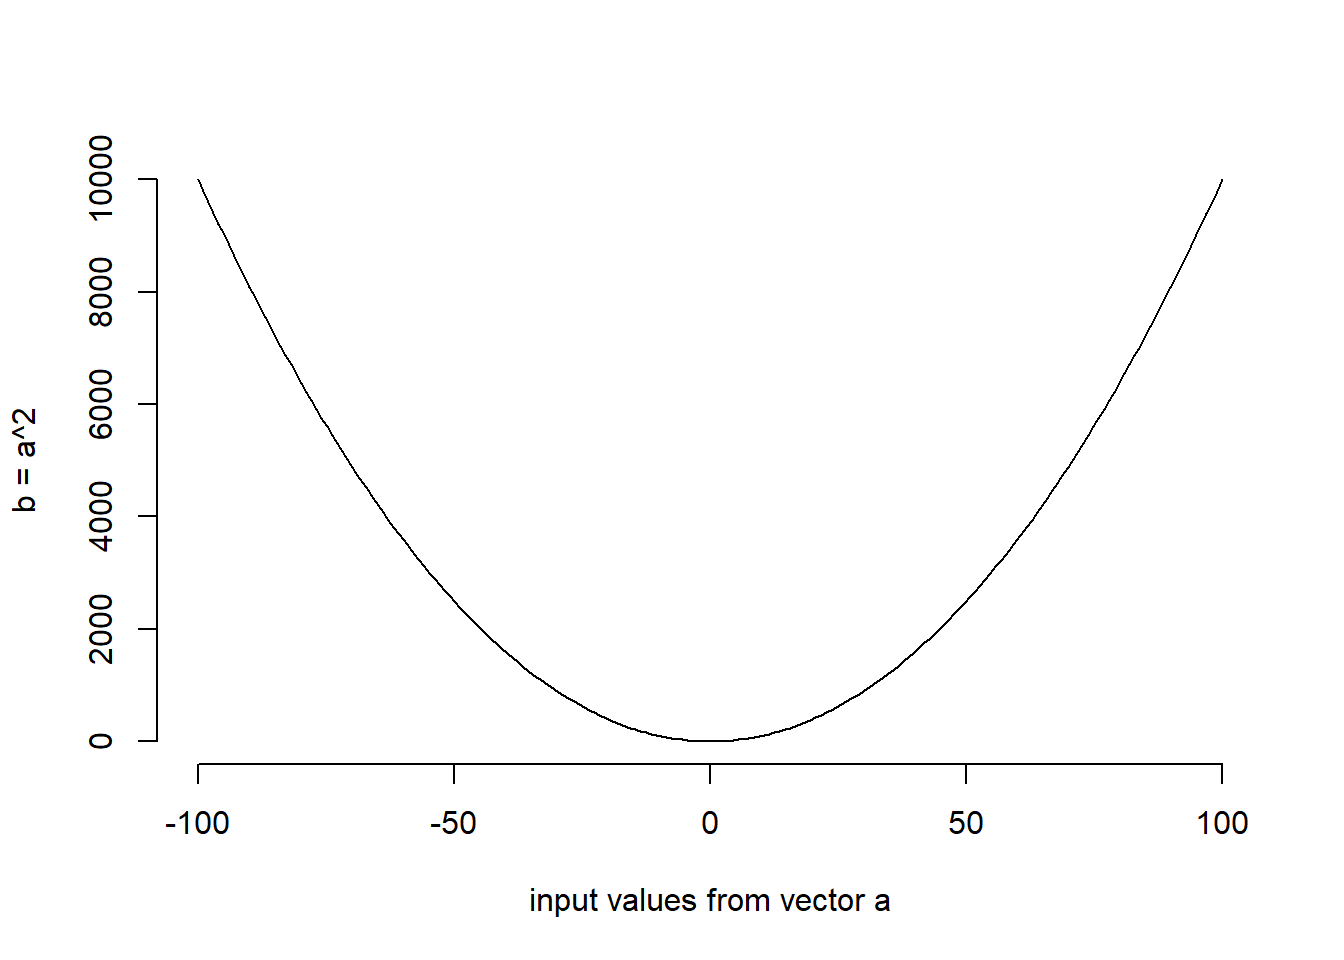
\includegraphics{statistics1_files/figure-latex/unnamed-chunk-43-1.pdf}

In this plot, you should see that the slope of the line increases, the
further we are from 0. We are taking individual differences from the
mean. Hence, if a value is exactly at the mean, the difference is zero.
The further, the value is from the mean (in any direction), the larger
the output value.

We will sum over the individual elements in the next step. Hence, values
that are further from the mean have a larger impact on the sum than
values that are closer to the mean.

In the next step, we take the sum over our squared deviations from the
mean

\begin{Shaded}
\begin{Highlighting}[]
\CommentTok{# sum over squared deviations vector}
\NormalTok{sum.of.squared.deviations <-}\StringTok{ }\KeywordTok{sum}\NormalTok{(squared.diffs.from.mean)}

\CommentTok{# print the sum}
\NormalTok{sum.of.squared.deviations}
\end{Highlighting}
\end{Shaded}

\begin{verbatim}
[1] 2151152127
\end{verbatim}

By summing over all elements of a vector, we end up with a scalar. The
sum is 2151152126.56.

We divide the sum of squared deviations by \(n-1\). Recall, that \(n\)
is the number of observations (elements in the vector) and \(-1\) is our
sample adjustment.

\begin{Shaded}
\begin{Highlighting}[]
\CommentTok{# get the variance}
\NormalTok{var.income <-}\StringTok{ }\NormalTok{sum.of.squared.deviations }\OperatorTok{/}\StringTok{ }\NormalTok{( }\KeywordTok{length}\NormalTok{(income) }\OperatorTok{-}\StringTok{ }\DecValTok{1}\NormalTok{ )}

\CommentTok{# print the variance}
\NormalTok{var.income}
\end{Highlighting}
\end{Shaded}

\begin{verbatim}
[1] 89631339
\end{verbatim}

The squared average deviation from mean income is 89631338.61.

In the last step, we take the square root over the variance to return to
our original units of income.

\begin{Shaded}
\begin{Highlighting}[]
\CommentTok{# get the standard deviation}
\KeywordTok{sqrt}\NormalTok{(var.income)}
\end{Highlighting}
\end{Shaded}

\begin{verbatim}
[1] 9467.383
\end{verbatim}

The average deviation from mean income in Berlin (24666.24) is 9467.38.

\subsection{Exercise 9}\label{exercise-9}

What is the level of measurement of the variable in the Sunday Question?

The variable measures vote choice. The answers are categories, the
parties, without any specific ordering. The level of measurement is
called categorical or nominal.

\subsection{Exercise 10}\label{exercise-10}

Take the most recent poll and describe what you see in terms of central
tendency and dispersion.

The most recent poll was carried out by Infratest/dimap on Thursday, 6
September. The most common value, the mode, is the appropriate measure
of central tendency. Christian Democrat (CDU/CSU) is the modal category.
Dispersion of a categorical variable is the proportion in each category
which we see displayed on the website:

\begin{longtable}[]{@{}ll@{}}
\toprule
Party & Proportion\tabularnewline
\midrule
\endhead
CDU/CSU & 0.29\tabularnewline
SPD & 0.18\tabularnewline
GREEN & 0.14\tabularnewline
FDP & 0.08\tabularnewline
THE LEFT & 0.10\tabularnewline
AFD & 0.16\tabularnewline
other & 0.05\tabularnewline
\bottomrule
\end{longtable}

\chapter{Research Design, Counterfactuals, Forming
Hypotheses}\label{research-design-counterfactuals-forming-hypotheses}

\section{Seminar}\label{seminar-1}

In today's seminar, we work with data frames (datasets). We will create
our own dataset, we subset datasets (access elements, rows and
variables). We load our first dataset into R. We also visualise data
using the \texttt{plot()} function. Finally, we estimate a treatment
effect in R---our first inference.

\subsection{setting up}\label{setting-up}

We set our working directory. R operates in specific directory (folder)
on our computer. We create a folder on our computer where we save our
scripts for our statistics 1 class. We name the folder \texttt{stats1}.
Let's create the folder on our computers now (in finder on Mac and
explorer on Windows).

Now, we set our working directory to the folder, we just created like
so:

\begin{figure}
\centering
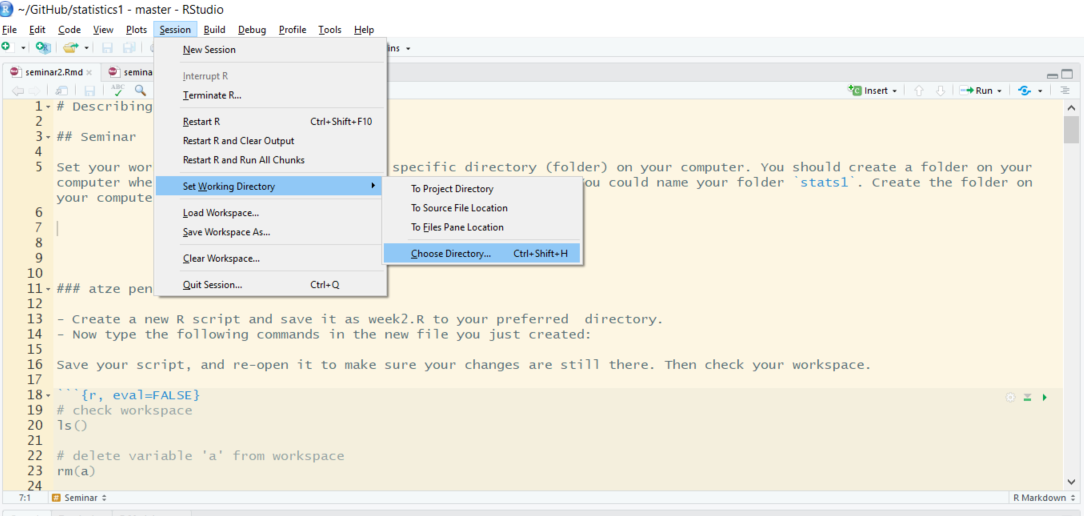
\includegraphics{./img/setwdir.png}
\caption{}
\end{figure}

Create a new R script and save it as week2.R to your \texttt{stats1}
directory. Now type the following commands in the new file you just
created:

\begin{Shaded}
\begin{Highlighting}[]
\CommentTok{# Create a numeric and a character variable}
\NormalTok{a <-}\StringTok{ }\DecValTok{5} \CommentTok{# numeric}
\NormalTok{a <-}\StringTok{ "five"} \CommentTok{# character}
\end{Highlighting}
\end{Shaded}

Save your script, and re-open it to make sure your changes are still
there. Then check your workspace.

\begin{Shaded}
\begin{Highlighting}[]
\CommentTok{# check workspace}
\KeywordTok{ls}\NormalTok{()}

\CommentTok{# delete variable 'a' from workspace}
\KeywordTok{rm}\NormalTok{(a)}

\CommentTok{# delete everything from workspace}
\KeywordTok{rm}\NormalTok{( }\DataTypeTok{list =} \KeywordTok{ls}\NormalTok{() )}

\CommentTok{# to clear console window press Crtl+l on Win or Command+l on Mac}
\end{Highlighting}
\end{Shaded}

\subsection{vectors and subsetting}\label{vectors-and-subsetting}

Last week we have already worked with vectors. We created a sequence for
example. This week, we learn about subsetting (accessing specific
elements of our vector).

We create a vector using the \texttt{c()} function, where c stands for
collect.

\begin{Shaded}
\begin{Highlighting}[]
\CommentTok{# Create a vector}
\NormalTok{my.vector <-}\StringTok{ }\KeywordTok{c}\NormalTok{(}\DecValTok{10}\NormalTok{,}\DecValTok{7}\NormalTok{,}\DecValTok{99}\NormalTok{,}\DecValTok{34}\NormalTok{,}\DecValTok{0}\NormalTok{,}\DecValTok{5}\NormalTok{) }\CommentTok{# a vector}
\NormalTok{my.vector}
\end{Highlighting}
\end{Shaded}

\begin{verbatim}
[1] 10  7 99 34  0  5
\end{verbatim}

Let's see how many elements our vector contains using the
\texttt{length()} function.

\begin{Shaded}
\begin{Highlighting}[]
\KeywordTok{length}\NormalTok{(my.vector) }\CommentTok{# how many elements?}
\end{Highlighting}
\end{Shaded}

\begin{verbatim}
[1] 6
\end{verbatim}

Next, we access the first element in our vector. We use square brackets
to access a specific element. The number in the square brackets is the
vector element that we access

\begin{Shaded}
\begin{Highlighting}[]
\CommentTok{# subsetting}
\NormalTok{my.vector[}\DecValTok{1}\NormalTok{] }\CommentTok{# 1st vector element}
\end{Highlighting}
\end{Shaded}

\begin{verbatim}
[1] 10
\end{verbatim}

To access all elements except the first element, we use the \texttt{-}
operator.

\begin{Shaded}
\begin{Highlighting}[]
\NormalTok{my.vector[}\OperatorTok{-}\DecValTok{1}\NormalTok{] }\CommentTok{# all elements but the 1st}
\end{Highlighting}
\end{Shaded}

\begin{verbatim}
[1]  7 99 34  0  5
\end{verbatim}

We can access elements 2 to 4 by using the colon.

\begin{Shaded}
\begin{Highlighting}[]
\NormalTok{my.vector[}\DecValTok{2}\OperatorTok{:}\DecValTok{4}\NormalTok{] }\CommentTok{# the 2nd to the 4th elements}
\end{Highlighting}
\end{Shaded}

\begin{verbatim}
[1]  7 99 34
\end{verbatim}

We can access two specific non-adjacent elements, by using the collect
function \texttt{c()}.

\begin{Shaded}
\begin{Highlighting}[]
\NormalTok{my.vector[}\KeywordTok{c}\NormalTok{(}\DecValTok{2}\NormalTok{,}\DecValTok{5}\NormalTok{)] }\CommentTok{# 2nd and 5th element}
\end{Highlighting}
\end{Shaded}

\begin{verbatim}
[1] 7 0
\end{verbatim}

No, we combine the \texttt{length()} function with the square brackets
to access the last element in our vector.

\begin{Shaded}
\begin{Highlighting}[]
\NormalTok{my.vector[}\KeywordTok{length}\NormalTok{(my.vector)] }\CommentTok{# the last element}
\end{Highlighting}
\end{Shaded}

\begin{verbatim}
[1] 5
\end{verbatim}

\subsection{data frames}\label{data-frames}

A data frame is an object that holds data in a tabular format similar to
how spreadsheets work. Variables are generally kept in columns and
observations are in rows.

Before we work with ready-made data, we create a small dataset
ourselves. It contains the populations of the sixteen German states. We
start with a vector that contains the names of those states. We call the
variable \emph{state}. Our variable shall contain text instead of
numbers. In R jargon, this is a character variable, sometimes referred
to as a string. Using quotes, we indicate that the variable type is
character. We use the \texttt{c()} function to create the vector.

\begin{Shaded}
\begin{Highlighting}[]
\CommentTok{# create a character vector containing state names}
\NormalTok{state <-}\StringTok{ }\KeywordTok{c}\NormalTok{(}
  \StringTok{"North Rhine-Westphalia"}\NormalTok{,}
  \StringTok{"Bavaria"}\NormalTok{,}
  \StringTok{"Baden-Wurttemberg"}\NormalTok{,}
  \StringTok{"Lower Saxony"}\NormalTok{,}
  \StringTok{"Hesse"}\NormalTok{,}
  \StringTok{"Saxony"}\NormalTok{,}
  \StringTok{"Rhineland-Palatinate"}\NormalTok{,}
  \StringTok{"Berlin"}\NormalTok{,}
  \StringTok{"Schleswig-Holstein"}\NormalTok{,}
  \StringTok{"Brandenburg"}\NormalTok{,}
  \StringTok{"Saxony-Anhalt"}\NormalTok{,}
  \StringTok{"Thuringia"}\NormalTok{,}
  \StringTok{"Hamburg"}\NormalTok{,}
  \StringTok{"Mecklenburg-Vorpommern"}\NormalTok{,}
  \StringTok{"Saarland"}\NormalTok{,}
  \StringTok{"Bremen"}
\NormalTok{  )}
\end{Highlighting}
\end{Shaded}

Now, we create a second variable for the populations. This is a numeric
vector, so we do not use the quotes.

\begin{Shaded}
\begin{Highlighting}[]
\NormalTok{population <-}\StringTok{ }\KeywordTok{c}\NormalTok{(}
  \DecValTok{17865516}\NormalTok{,}
  \DecValTok{12843514}\NormalTok{,}
  \DecValTok{10879618}\NormalTok{,}
  \DecValTok{7926599}\NormalTok{,}
  \DecValTok{6176172}\NormalTok{,}
  \DecValTok{4084851}\NormalTok{,}
  \DecValTok{4052803}\NormalTok{,}
  \DecValTok{3670622}\NormalTok{,}
  \DecValTok{2858714}\NormalTok{,}
  \DecValTok{2484826}\NormalTok{,}
  \DecValTok{2245470}\NormalTok{,}
  \DecValTok{2170714}\NormalTok{,}
  \DecValTok{1787408}\NormalTok{,}
  \DecValTok{1612362}\NormalTok{,}
  \DecValTok{995597}\NormalTok{,}
  \DecValTok{671489}
\NormalTok{)}
\end{Highlighting}
\end{Shaded}

Now with both vectors created, we combine them into a dataframe. We put
our vectors in and give them names. In this case the variable names in
the dataset correspond to our vector names. The name goes in front of
the equal sign and the vector object name, after.

\begin{Shaded}
\begin{Highlighting}[]
\NormalTok{popdata <-}\StringTok{ }\KeywordTok{data.frame}\NormalTok{( }
  \DataTypeTok{state =}\NormalTok{ state,}
  \DataTypeTok{population =}\NormalTok{ population}
\NormalTok{  )}
\end{Highlighting}
\end{Shaded}

You should see the new data frame object in your global environment
window. You can view the dataset in the spreadsheet form that we are all
used to by clicking on the oject name.

We can see the names of variables in our dataset with the names function

\begin{Shaded}
\begin{Highlighting}[]
\KeywordTok{names}\NormalTok{(popdata)}
\end{Highlighting}
\end{Shaded}

\begin{verbatim}
[1] "state"      "population"
\end{verbatim}

Let's check the variable types in our data using the \texttt{str()}
function.

\begin{Shaded}
\begin{Highlighting}[]
\KeywordTok{str}\NormalTok{(popdata)}
\end{Highlighting}
\end{Shaded}

\begin{verbatim}
'data.frame':   16 obs. of  2 variables:
 $ state     : Factor w/ 16 levels "Baden-Wurttemberg",..: 10 2 1 8 7 13 11 3 15 4 ...
 $ population: num  17865516 12843514 10879618 7926599 6176172 ...
\end{verbatim}

The variable \emph{state} is a factor variable. R has turned the
character variable into a categorical variable automatically. The
variable \emph{population} is numeric. These variable types differ. We
can calculate with numeric variables only.

Often we want to access certain observations (rows) or certain columns
(variables) or a combination of the two without looking at the entire
dataset all at once. We can use square brackets to subset data frames.
In square brackets we put a row and a column coordinate separated by a
comma. The row coordinate goes first and the column coordinate second.
So \texttt{popdata{[}10,\ 2{]}} returns the 10th row and second column
of the data frame. If we leave the column coordinate empty this means we
would like all columns. So, \texttt{popdata{[}10,{]}} returns the 10th
row of the dataset. If we leave the row coordinate empty, R returns the
entire column. \texttt{popdata{[},2{]}} returns the second column of the
dataset.

We can look at the first five rows of a dataset to get a better
understanding of it with the colon in brackets like so:
\texttt{popdata{[}1:5,{]}}. We could display the second and fifth
columns of the dataset by using the \texttt{c()} function in brackets
like so: \texttt{popdata{[},\ c(2,5){]}}.

It's your turn. Display all columns of the popdata dataset and show rows
10 to 15. Next display all columns of the dataset and rows 4 and 7.

\begin{Shaded}
\begin{Highlighting}[]
\NormalTok{popdata[}\DecValTok{10}\OperatorTok{:}\DecValTok{15}\NormalTok{, ] }\CommentTok{# elements in 10th to 15th row, all columns}
\end{Highlighting}
\end{Shaded}

\begin{verbatim}
                    state population
10            Brandenburg    2484826
11          Saxony-Anhalt    2245470
12              Thuringia    2170714
13                Hamburg    1787408
14 Mecklenburg-Vorpommern    1612362
15               Saarland     995597
\end{verbatim}

\begin{Shaded}
\begin{Highlighting}[]
\NormalTok{popdata[}\KeywordTok{c}\NormalTok{(}\DecValTok{4}\NormalTok{, }\DecValTok{7}\NormalTok{), ] }\CommentTok{# elements in 4th and 7th row, all column}
\end{Highlighting}
\end{Shaded}

\begin{verbatim}
                 state population
4         Lower Saxony    7926599
7 Rhineland-Palatinate    4052803
\end{verbatim}

In order to access individual columns of a data frame we can also use
the dollar sign \texttt{\$}. For example, let's see how to access the
\texttt{population} column.

\begin{Shaded}
\begin{Highlighting}[]
\NormalTok{popdata}\OperatorTok{$}\NormalTok{population}
\end{Highlighting}
\end{Shaded}

\begin{verbatim}
 [1] 17865516 12843514 10879618  7926599  6176172  4084851  4052803
 [8]  3670622  2858714  2484826  2245470  2170714  1787408  1612362
[15]   995597   671489
\end{verbatim}

Now, access the state column.

\begin{Shaded}
\begin{Highlighting}[]
\NormalTok{popdata}\OperatorTok{$}\NormalTok{state}
\end{Highlighting}
\end{Shaded}

\begin{verbatim}
 [1] North Rhine-Westphalia Bavaria                Baden-Wurttemberg     
 [4] Lower Saxony           Hesse                  Saxony                
 [7] Rhineland-Palatinate   Berlin                 Schleswig-Holstein    
[10] Brandenburg            Saxony-Anhalt          Thuringia             
[13] Hamburg                Mecklenburg-Vorpommern Saarland              
[16] Bremen                
16 Levels: Baden-Wurttemberg Bavaria Berlin Brandenburg Bremen ... Thuringia
\end{verbatim}

\subsection{Loading data}\label{loading-data}

Before you load the dataset into R, you first download it and save it
locally in your \texttt{Stats1} folder. Download the data
\href{http://philippbroniecki.github.io/ML2017.io/data/BSAS_manip.RData}{here}.

We often load existing data sets into R for analysis. Data come in many
different file formats such as \texttt{.csv}, \texttt{.tab},
\texttt{.dta}, etc. Today we will load a dataset which is stored in R's
native file format: \texttt{.RData}. The function to load data from this
file format is called: \texttt{load()}. If you managed to set your
working directory correctly just now
(\texttt{setwd("\textasciitilde{}/Stats1"})), then you should just be
able to run the line of code below.

We load the dataset with the \texttt{load()} function:

\begin{Shaded}
\begin{Highlighting}[]
\CommentTok{# load perception of non-western foreigners data}
\KeywordTok{load}\NormalTok{(}\StringTok{"BSAS_manip.RData"}\NormalTok{)}
\end{Highlighting}
\end{Shaded}

The non-western foreingers data is about the subjective perception of
immigrants from non-western countries. The perception of immigrants from
a context that is not similar to the one's own ,is often used as a proxy
for racism. Whether this is a fair measure or not is debatable but let's
examine the data from a survey carried out in Britain.

Let's check the codebook of our data.

\begin{tabular}{l|l}
\hline
Variable & Description\\
\hline
IMMBRIT & Out of every 100 people in Britain, how many do you think are immigrants from non-western countries?\\
\hline
over.estimate & 1 if estimate is higher than 10.7\%.\\
\hline
RSex & 1 = male, 2 = female\\
\hline
RAge & Age of respondent\\
\hline
Househld & Number of people living in respondent's household\\
\hline
party identification & 1 = Conservatives, 2 = Labour, 3 = SNP, 4 = Greens, 5 = Ukip, 6 = BNP, 7 = other\\
\hline
paper & Do you normally read any daily morning newspaper 3+ times/week?\\
\hline
WWWhourspW & How many hours WWW per week?\\
\hline
religious & Do you regard yourself as belonging to any particular religion?\\
\hline
employMonths & How many mnths w. present employer?\\
\hline
urban & Population density, 4 categories (highest density is 4, lowest is 1)\\
\hline
health.good & How is your health in general for someone of your age? (0: bad, 1: fair, 2: fairly good, 3: good)\\
\hline
HHInc & Income bands for household, high number = high HH income\\
\hline
\end{tabular}

We can look at the variable names in our data with the
\href{http://bit.ly/R_names}{\texttt{names()}} function.

The \href{http://bit.ly/R_dim}{\texttt{dim()}} function can be used to
find out the dimensions of the dataset (dimension 1 = rows, dimension 2
= columns).

\begin{Shaded}
\begin{Highlighting}[]
\KeywordTok{dim}\NormalTok{(data2)}
\end{Highlighting}
\end{Shaded}

\begin{verbatim}
[1] 1049   19
\end{verbatim}

So, the \href{http://bit.ly/R_dim}{\texttt{dim()}} function tells us
that we have data from 1049 respondents with 19 variables for each
respondent.

Let's take a quick peek at the first 10 observations to see what the
dataset looks like. By default the
\href{http://bit.ly/R_head}{\texttt{head()}} function returns the first
6 rows, but let's tell it to return the first 10 rows instead.

\begin{Shaded}
\begin{Highlighting}[]
\KeywordTok{head}\NormalTok{(data2, }\DataTypeTok{n =} \DecValTok{10}\NormalTok{)}
\end{Highlighting}
\end{Shaded}

\begin{verbatim}
   IMMBRIT over.estimate RSex RAge Househld Cons Lab SNP Ukip BNP GP
1        1             0    1   50        2    0   1   0    0   0  0
2       50             1    2   18        3    0   0   0    0   0  0
3       50             1    2   60        1    0   0   0    0   0  0
4       15             1    2   77        2    0   0   0    0   0  0
5       20             1    2   67        1    0   0   0    0   0  0
6       30             1    1   30        4    0   0   0    0   0  0
7       60             1    2   56        2    0   0   1    0   0  0
8        7             0    1   49        1    0   0   0    0   0  0
9       30             1    1   40        4    0   0   1    0   0  0
10       2             0    1   61        3    1   0   0    0   0  0
   party.other paper WWWhourspW religious employMonths urban health.good
1            0     0          1         0           72     4           1
2            1     0          4         0           72     4           2
3            1     0          1         0          456     3           3
4            1     1          2         1           72     1           3
5            1     0          1         1           72     3           3
6            1     1         14         0           72     1           2
7            0     0          5         1          180     1           2
8            1     1          8         0          156     4           2
9            0     0          3         1          264     2           2
10           0     1          0         1           72     1           3
   HHInc
1     13
2      3
3      9
4      8
5      9
6      9
7     13
8     14
9     11
10     8
\end{verbatim}

\subsection{Plots}\label{plots}

We can visualize the data with the help of a boxplot, so let's see how
the perception of the number of immigrants is distributed.

\begin{Shaded}
\begin{Highlighting}[]
\CommentTok{# how good are we at guessing immigration}
\KeywordTok{boxplot}\NormalTok{(}
\NormalTok{  data2}\OperatorTok{$}\NormalTok{IMMBRIT, }
  \DataTypeTok{main =} \StringTok{"Perception of Immigration from Non-Western Countries"}\NormalTok{,}
  \DataTypeTok{ylab =} \StringTok{"Subjective number of immigrants per 100 British"}\NormalTok{, }
  \DataTypeTok{frame.plot =} \OtherTok{FALSE}\NormalTok{, }\DataTypeTok{col =} \StringTok{"darkgray"}
\NormalTok{  )}
\end{Highlighting}
\end{Shaded}

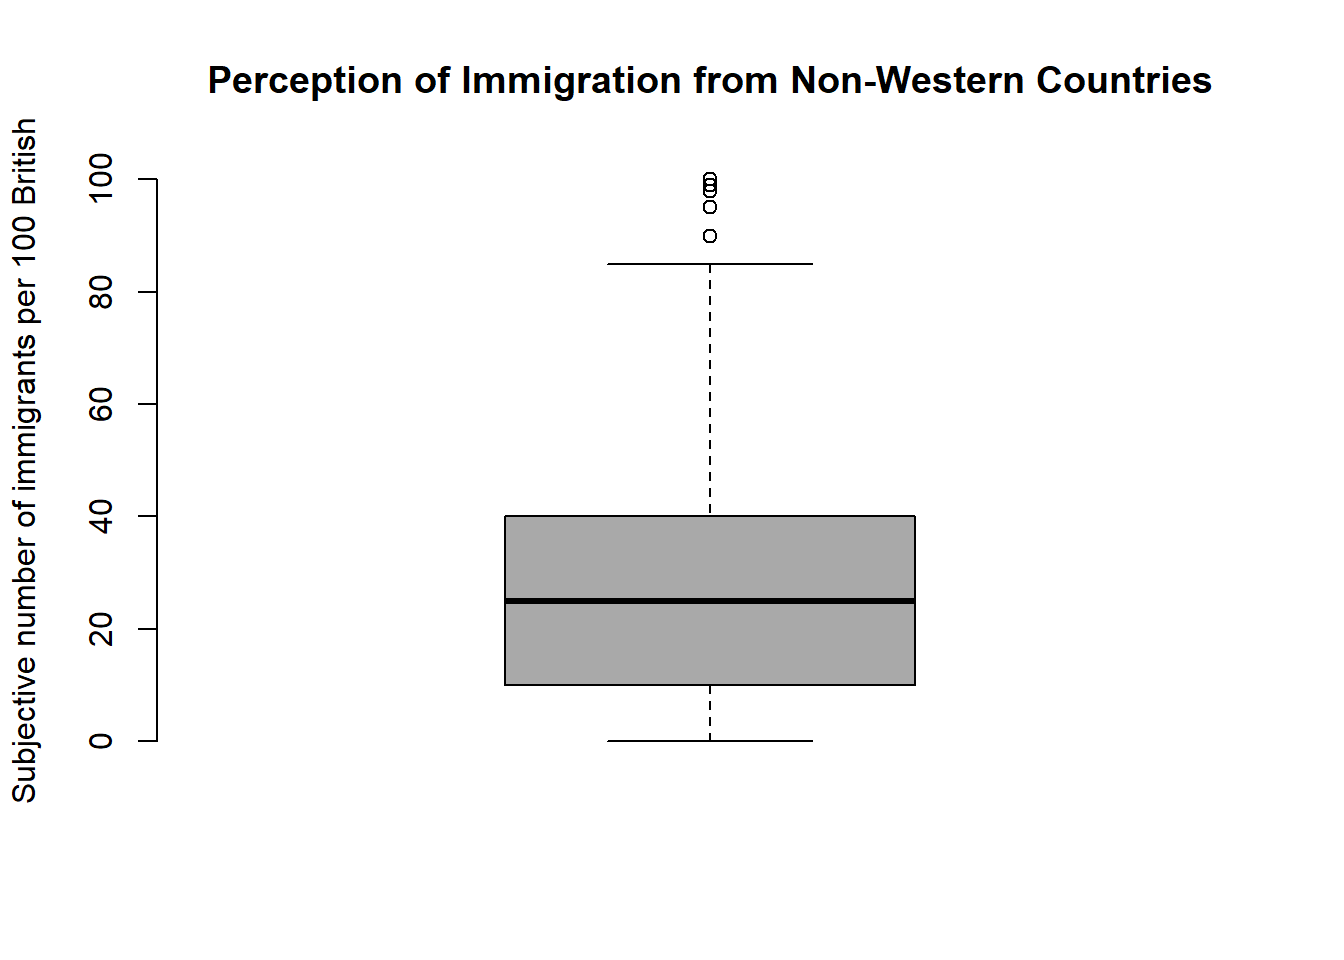
\includegraphics{statistics1_files/figure-latex/unnamed-chunk-69-1.pdf}

Notice how the lower whisker is much shorter than the upper one. The
distribution is right skewed. The right tail (higher values) is a lot
longer. We can see this beter using a density plot. We combine R's
\texttt{denisty()} function with the \texttt{plot()} function.

\begin{Shaded}
\begin{Highlighting}[]
\KeywordTok{plot}\NormalTok{(}
  \KeywordTok{density}\NormalTok{(data2}\OperatorTok{$}\NormalTok{IMMBRIT),}
  \DataTypeTok{bty =} \StringTok{"n"}\NormalTok{,}
  \DataTypeTok{main =} \StringTok{"Perception of Immigration from Non-Western Countries"}\NormalTok{,}
  \DataTypeTok{xlab =} \StringTok{"Subjective number of immigrants per 100 British"}
\NormalTok{  )}
\end{Highlighting}
\end{Shaded}

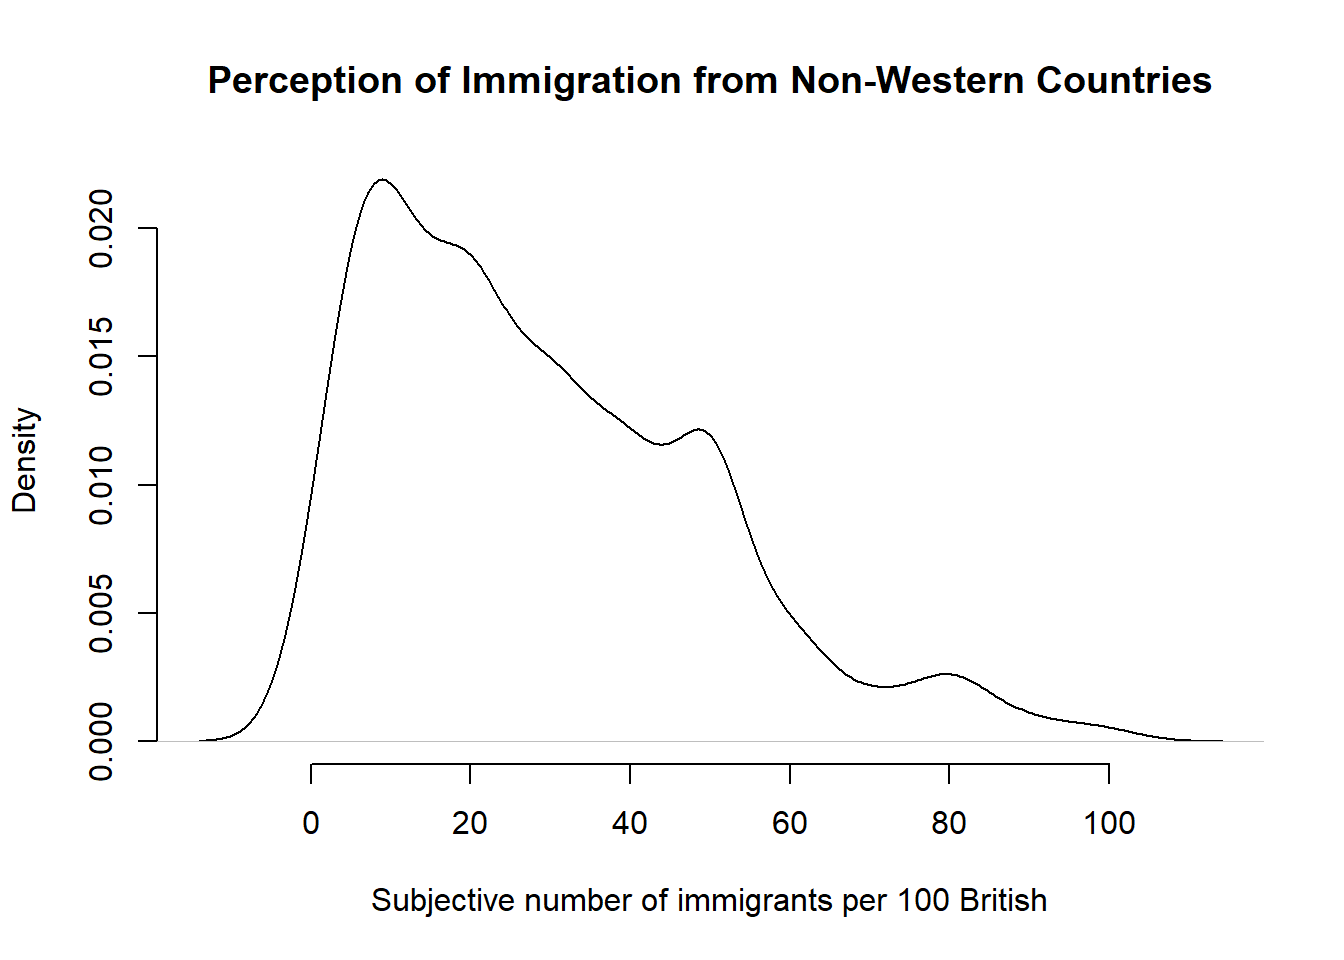
\includegraphics{statistics1_files/figure-latex/unnamed-chunk-70-1.pdf}

We can also plot histograms using the \texttt{hist()} function.

\begin{Shaded}
\begin{Highlighting}[]
\CommentTok{# histogram}
\KeywordTok{hist}\NormalTok{( data2}\OperatorTok{$}\NormalTok{employMonths, }\DataTypeTok{main =} \StringTok{"histogram"}\NormalTok{)}
\end{Highlighting}
\end{Shaded}

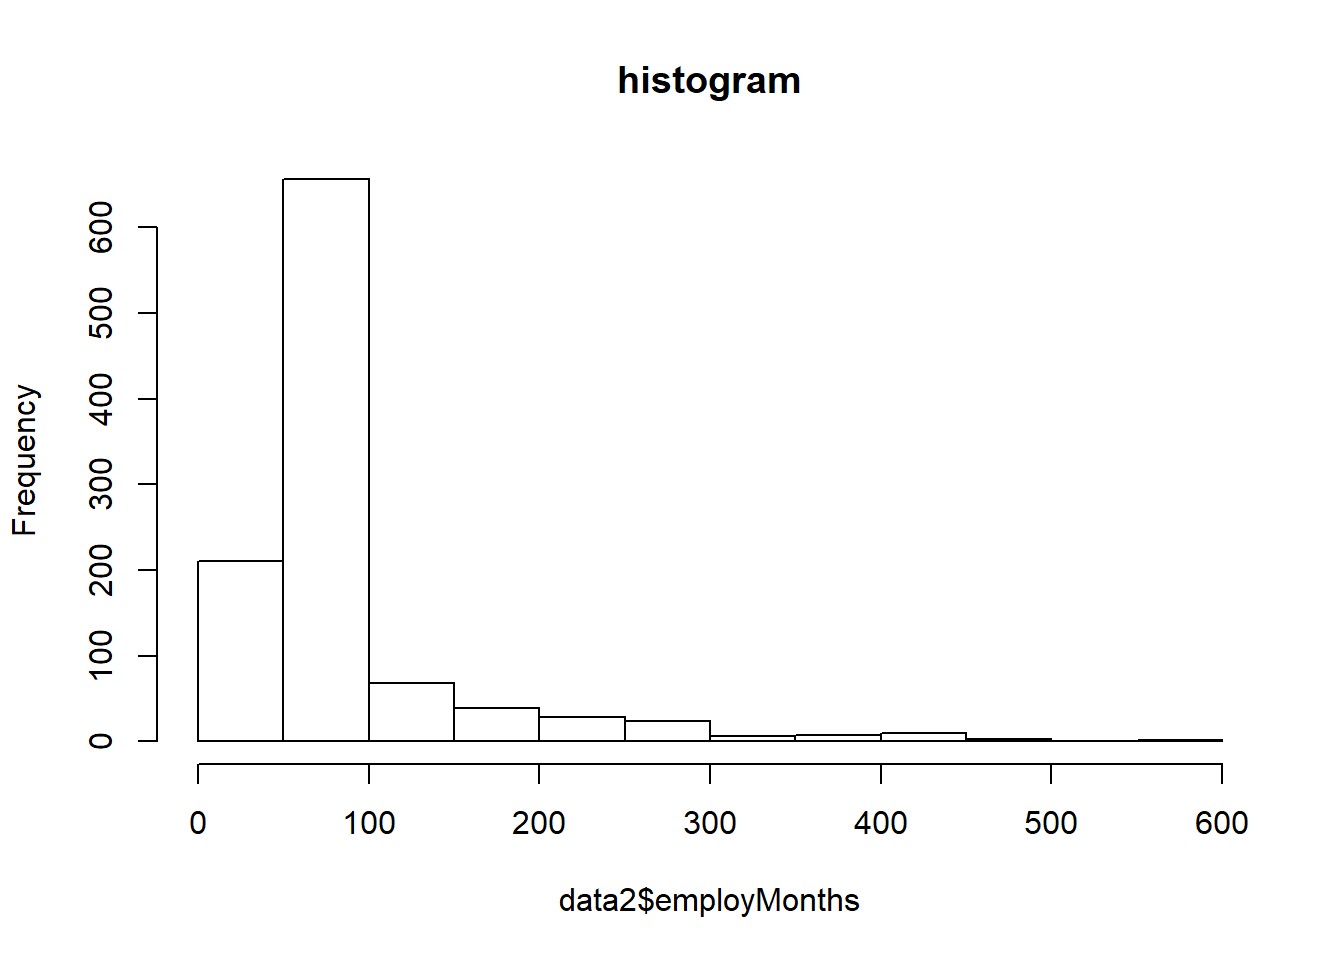
\includegraphics{statistics1_files/figure-latex/unnamed-chunk-71-1.pdf}

It is plausible that perception of immigration from Non-Western
countries is related to party affiliation. In our dataset, we have a
some party affiliation dummies (binary variables). We can use square
brackets to subset our data such that we produce a boxplot only for
members of the Conservative Party. We have a look at the variable
\emph{Cons} using the \texttt{table()} function first.

\begin{Shaded}
\begin{Highlighting}[]
\KeywordTok{table}\NormalTok{(data2}\OperatorTok{$}\NormalTok{Cons)}
\end{Highlighting}
\end{Shaded}

\begin{verbatim}

  0   1 
765 284 
\end{verbatim}

In our data, 284 respondents associate with the Conservative party and
765 do not. We create a boxplot of \emph{IMMBRIT} but only for members
of the Conservative Party. We do so by using the square brackets to
subset our data.

\begin{Shaded}
\begin{Highlighting}[]
\CommentTok{# boxplot of immbrit for those observations where Cons is 1}
\KeywordTok{boxplot}\NormalTok{(}
\NormalTok{  data2}\OperatorTok{$}\NormalTok{IMMBRIT[data2}\OperatorTok{$}\NormalTok{Cons}\OperatorTok{==}\DecValTok{1}\NormalTok{],}
  \DataTypeTok{frame.plot =} \OtherTok{FALSE}\NormalTok{,}
  \DataTypeTok{xlab =} \StringTok{"Conservatives"}\NormalTok{,}
  \DataTypeTok{col =} \StringTok{"blue"}
\NormalTok{  )}
\end{Highlighting}
\end{Shaded}

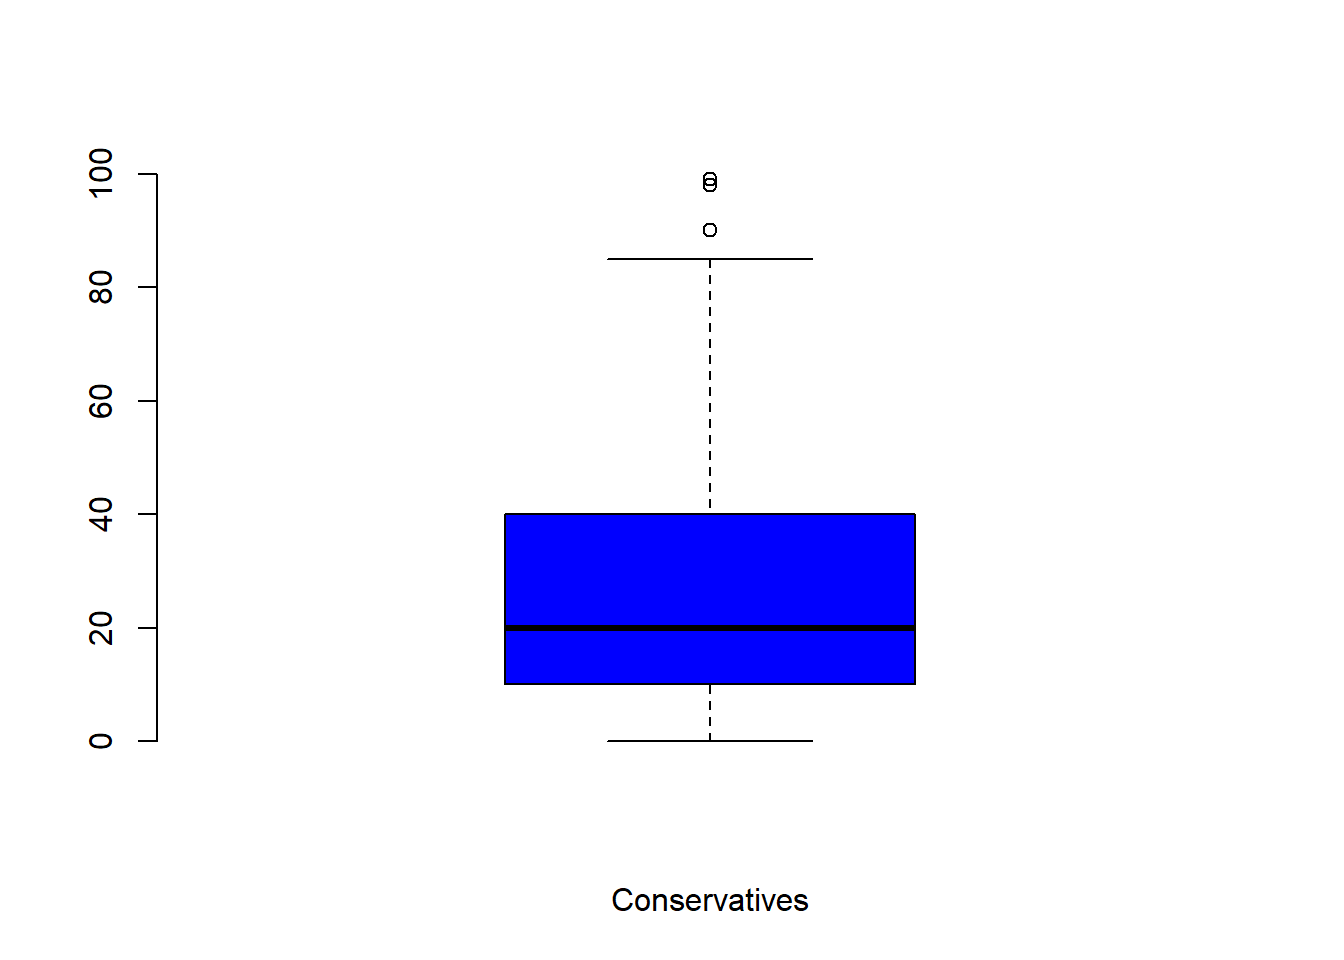
\includegraphics{statistics1_files/figure-latex/unnamed-chunk-73-1.pdf}

We would now like to compare the distribution of the perception fo
Conservatives to the distribution among Labour respondents. We can
subset the data just like we did for the Conservative Party. In addtion,
we want to plot the two plots next to each other, i.e., they should be
in the same plot. We can achieve this with the \texttt{par()} function
and the \texttt{mfrow} argument. This will spilt the plot window into
rows and columns. We want 2 columns to plot 2 boxplots next to each
other.

\begin{Shaded}
\begin{Highlighting}[]
\CommentTok{# split plot window into 1 row and 2 columns}
\KeywordTok{par}\NormalTok{(}\DataTypeTok{mfrow =} \KeywordTok{c}\NormalTok{(}\DecValTok{1}\NormalTok{,}\DecValTok{2}\NormalTok{))}

\CommentTok{# plot 1}
\KeywordTok{boxplot}\NormalTok{(}
\NormalTok{  data2}\OperatorTok{$}\NormalTok{IMMBRIT[data2}\OperatorTok{$}\NormalTok{Cons}\OperatorTok{==}\DecValTok{1}\NormalTok{],}
  \DataTypeTok{frame.plot =} \OtherTok{FALSE}\NormalTok{,}
  \DataTypeTok{xlab =} \StringTok{"Conservatives"}\NormalTok{,}
  \DataTypeTok{col =} \StringTok{"blue"}
\NormalTok{  )}

\CommentTok{# plot 2}
\KeywordTok{boxplot}\NormalTok{(}
\NormalTok{  data2}\OperatorTok{$}\NormalTok{IMMBRIT[data2}\OperatorTok{$}\NormalTok{Lab}\OperatorTok{==}\DecValTok{1}\NormalTok{],}
  \DataTypeTok{frame.plot =} \OtherTok{FALSE}\NormalTok{,}
  \DataTypeTok{xlab =} \StringTok{"Labour"}\NormalTok{,}
  \DataTypeTok{col =} \StringTok{"red"}
\NormalTok{  )}
\end{Highlighting}
\end{Shaded}

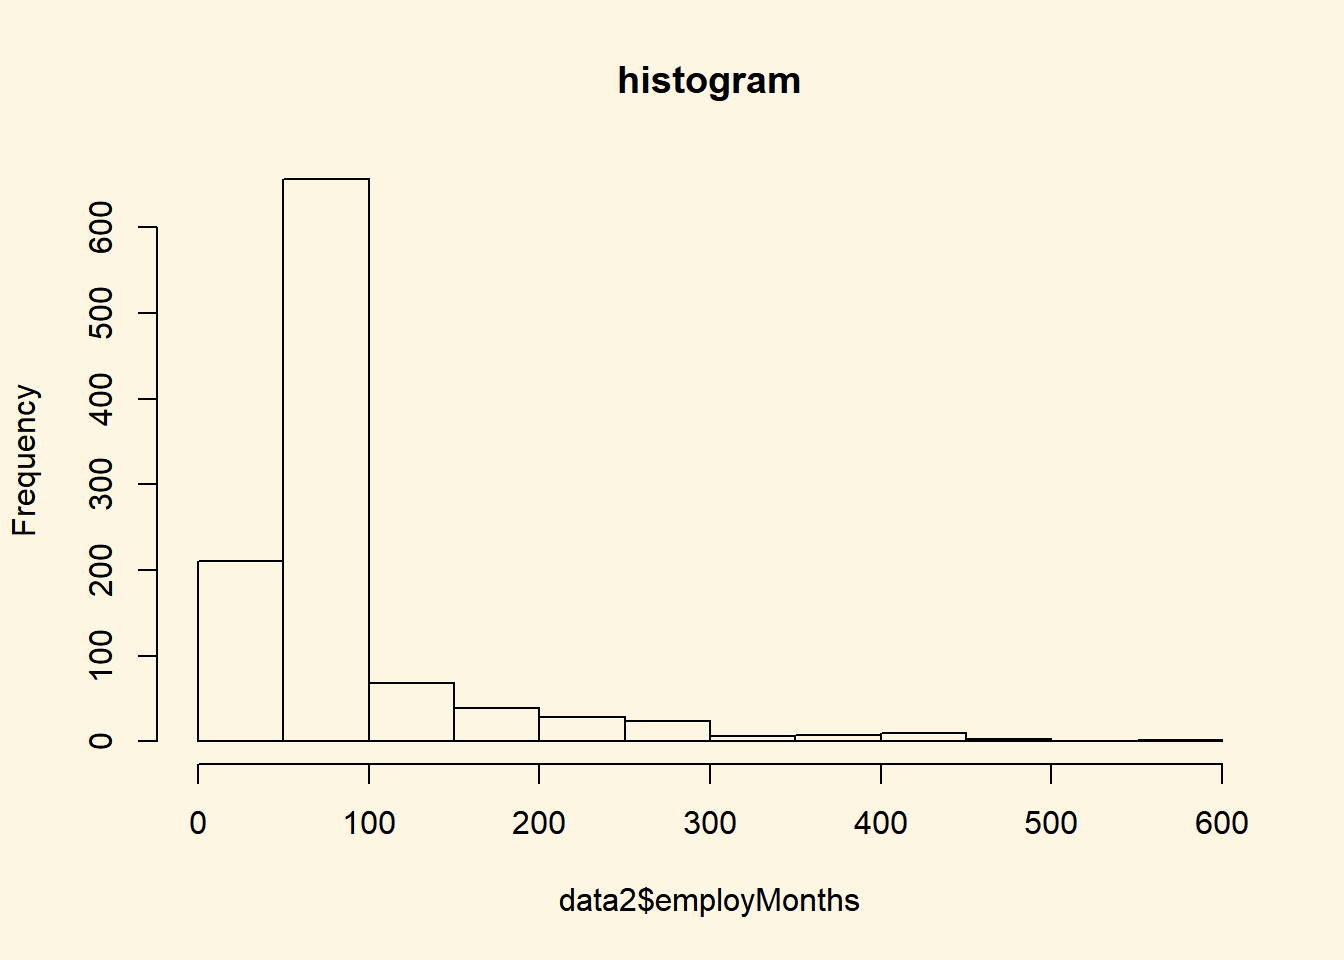
\includegraphics{statistics1_files/figure-latex/unnamed-chunk-74-1.pdf}

It is very hard to spot differences. The distributions are similar. The
median for Labour respondents is larger which mean that the central
Labour respondent over-estimates immigration more than the central
Conservative respondent.

You can play around with the non-western foreigners data on your own
time. We now turn to a dataset that is integrated in R already. It is
called \texttt{longley}. Use the \texttt{help()} function to see what
this dataset is about.

\begin{Shaded}
\begin{Highlighting}[]
\KeywordTok{help}\NormalTok{(longley)}
\end{Highlighting}
\end{Shaded}

\begin{verbatim}
starting httpd help server ... done
\end{verbatim}

Let's create a scatterplot with the \texttt{Year} variable on the x-axis
and \texttt{Employed} on the y-axis.

\begin{Shaded}
\begin{Highlighting}[]
\KeywordTok{plot}\NormalTok{(}\DataTypeTok{x =}\NormalTok{ longley}\OperatorTok{$}\NormalTok{Year, }\CommentTok{# x-axis variable}
     \DataTypeTok{y =}\NormalTok{ longley}\OperatorTok{$}\NormalTok{Employed, }\CommentTok{# y-axis variable}
     \DataTypeTok{bty =} \StringTok{"n"} \CommentTok{# no box around the plot}
\NormalTok{     )}
\end{Highlighting}
\end{Shaded}

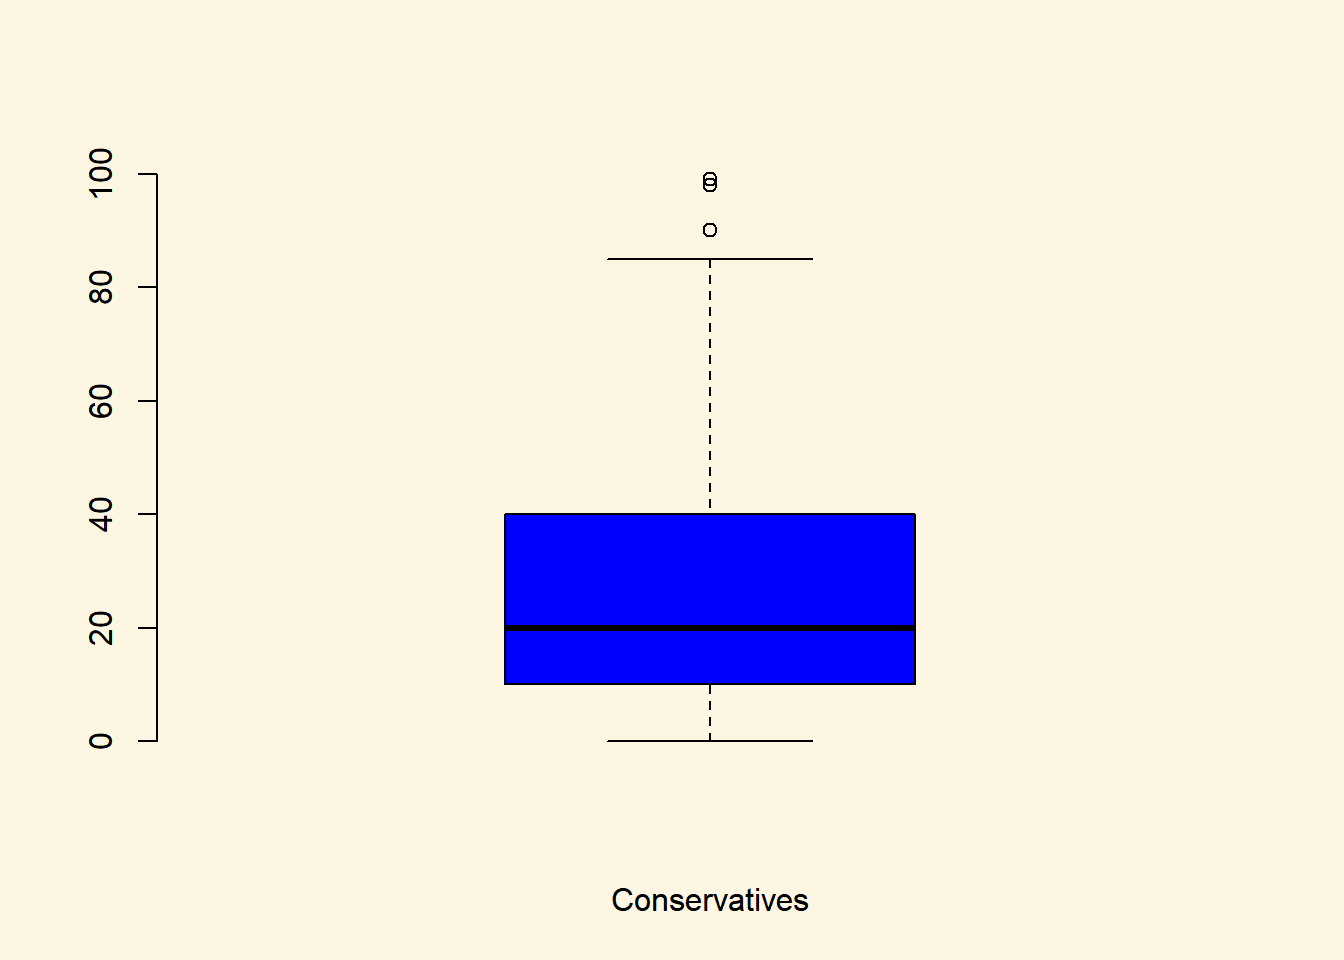
\includegraphics{statistics1_files/figure-latex/unnamed-chunk-76-1.pdf}

To create a line plot instead, we use the same function with one
additional argument \texttt{type\ =\ "l"}.

\begin{Shaded}
\begin{Highlighting}[]
\KeywordTok{plot}\NormalTok{(longley}\OperatorTok{$}\NormalTok{Year, longley}\OperatorTok{$}\NormalTok{Employed, }\DataTypeTok{type =} \StringTok{"l"}\NormalTok{)}
\end{Highlighting}
\end{Shaded}

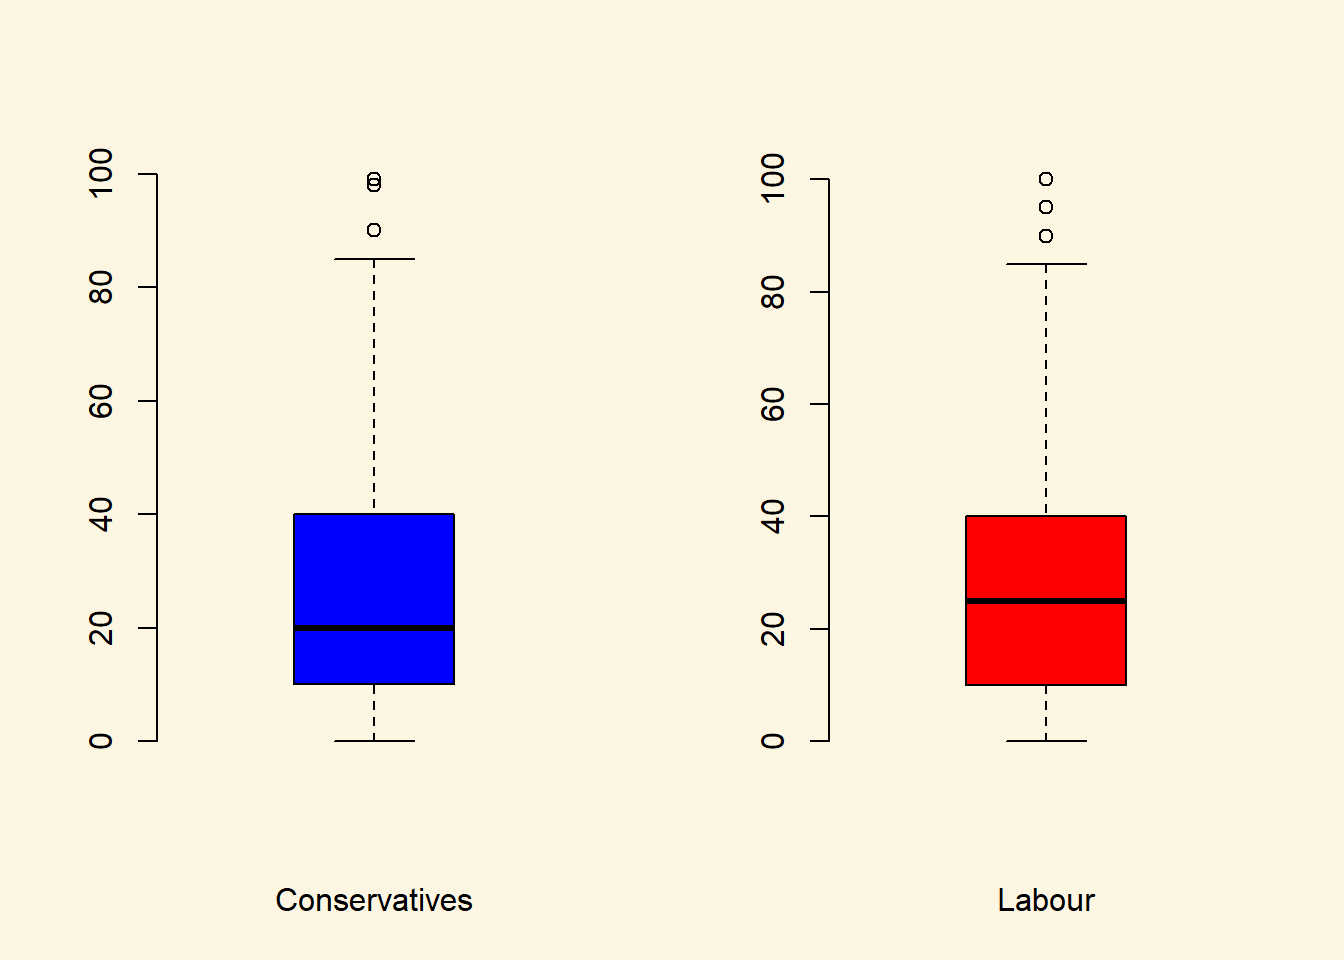
\includegraphics{statistics1_files/figure-latex/unnamed-chunk-77-1.pdf}

Create a plot that includes both points and lines.

\begin{Shaded}
\begin{Highlighting}[]
\KeywordTok{plot}\NormalTok{(longley}\OperatorTok{$}\NormalTok{Year, longley}\OperatorTok{$}\NormalTok{Employed, }\DataTypeTok{type =} \StringTok{"b"}\NormalTok{)}
\end{Highlighting}
\end{Shaded}

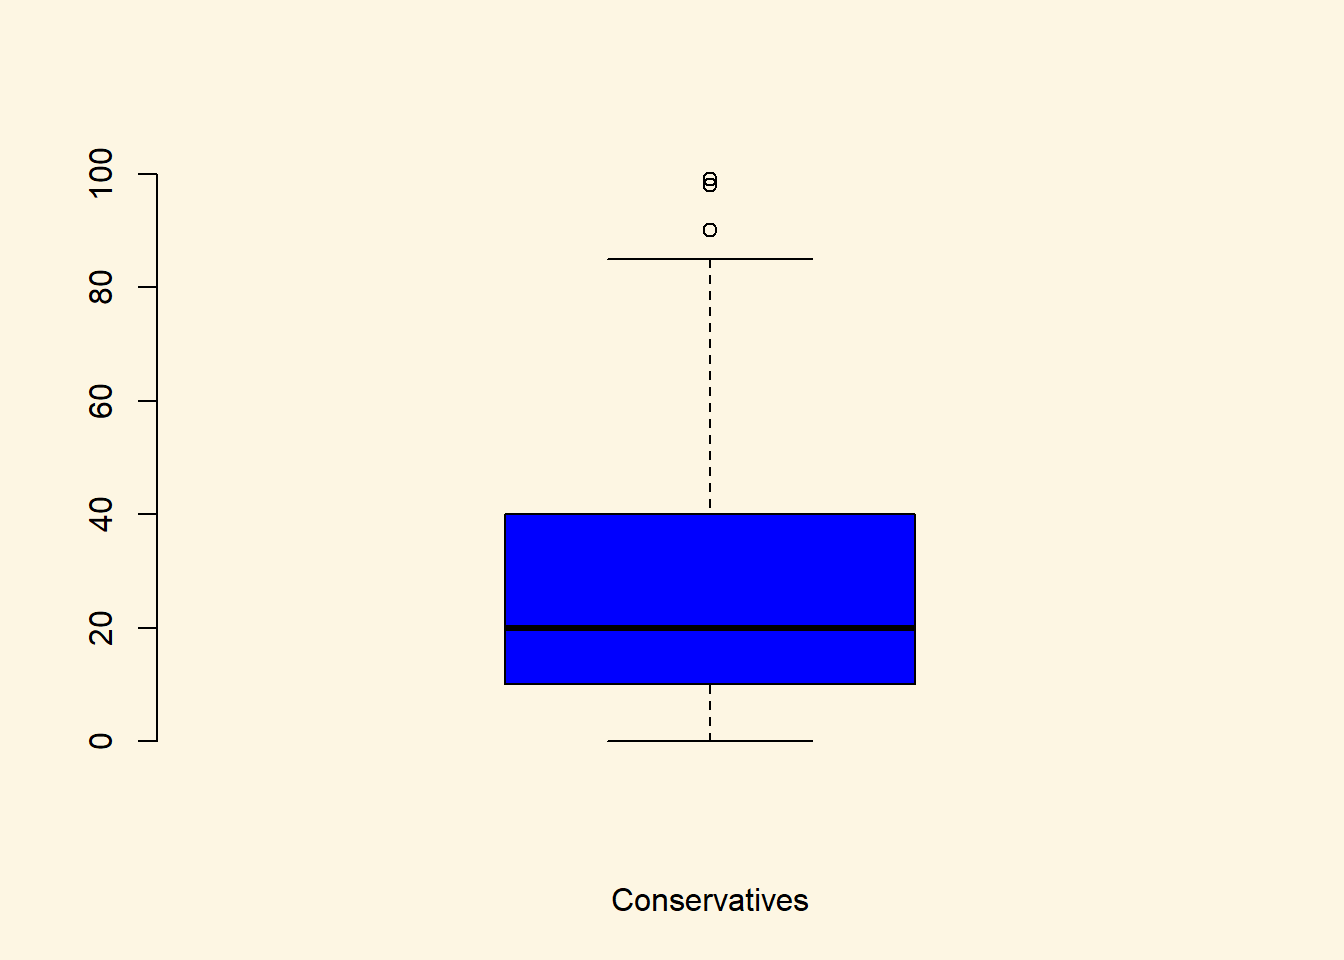
\includegraphics{statistics1_files/figure-latex/unnamed-chunk-78-1.pdf}

\subsection{Average Treatment Effect}\label{average-treatment-effect}

In the lecture, we estimated the average treatment effect on a small
example. We will do this again here. Recall, that the average treatment
effect is the difference between two means.

Let's suppose, associating with right-wing parties causes people to
over-estimate the number of non-western foreigners. Our treatment
variable is whether a respondent assoicates with the UK Independence
Party. It is 1 if that is the case and 0 otherwise. Let's inspect the
variable \emph{Ukip}.

\begin{Shaded}
\begin{Highlighting}[]
\KeywordTok{table}\NormalTok{(data2}\OperatorTok{$}\NormalTok{Ukip)}
\end{Highlighting}
\end{Shaded}

\begin{verbatim}

   0    1 
1018   31 
\end{verbatim}

31 respondents identify with Ukip.

The average treatment effect, as we learned, would be the difference
between the mean outcomes for those who received the treament minus the
mean for those who did not reicive the treatment.

We have all the tools to solve the problem. Let's take the mean of the
treated group first.

\begin{Shaded}
\begin{Highlighting}[]
\NormalTok{mean.y.treated <-}\StringTok{ }\KeywordTok{mean}\NormalTok{(data2}\OperatorTok{$}\NormalTok{IMMBRIT[data2}\OperatorTok{$}\NormalTok{Ukip }\OperatorTok{==}\StringTok{ }\DecValTok{1}\NormalTok{])}
\NormalTok{mean.y.treated}
\end{Highlighting}
\end{Shaded}

\begin{verbatim}
[1] 24.29032
\end{verbatim}

The double equal sign \texttt{==} is a logical operator and means ``is
equal to''. R returns true or false depending on whether the respondent
does identify with Ukip or not. The mean of \emph{IMMBRIT} is then
computed only for respondents who accociate with Ukip.

Let's take the mean of the second group, the untreated group.

\begin{Shaded}
\begin{Highlighting}[]
\NormalTok{mean.y.untreated <-}\StringTok{ }\KeywordTok{mean}\NormalTok{(data2}\OperatorTok{$}\NormalTok{IMMBRIT[data2}\OperatorTok{$}\NormalTok{Ukip }\OperatorTok{==}\StringTok{ }\DecValTok{0}\NormalTok{])}
\NormalTok{mean.y.untreated}
\end{Highlighting}
\end{Shaded}

\begin{verbatim}
[1] 29.17485
\end{verbatim}

The treatment effect is the difference in means:

\begin{Shaded}
\begin{Highlighting}[]
\NormalTok{mean.y.treated }\OperatorTok{-}\StringTok{ }\NormalTok{mean.y.untreated}
\end{Highlighting}
\end{Shaded}

\begin{verbatim}
[1] -4.88453
\end{verbatim}

The result is surprising. Ukip members over-estimate the number of
non-western foreigners less members of all other paries. Our claim is
not quite supported by the data. We should be very careful with these
results, however. We used experimental language but our data is
observational. A multitude of confounders could bias our estimate of the
causal effect.

\subsection{Exercises}\label{exercises-1}

\begin{enumerate}
\def\labelenumi{\arabic{enumi}.}
\tightlist
\item
  Create a script and call it assignment02. Save your script.
\item
  Use the \texttt{names()} function to display the variable names of the
  \texttt{longley} dataset.
\item
  Use square brackets to access the 4th column of the dataset.
\item
  Use the dollar sign to access the 4th column of the dataset.
\item
  Access the two cells from row 4 and column 1 and row 6 and column 3.
\item
  Using the \texttt{longley} data produce a line plot with GNP on the
  y-axis and population on the x-axis.
\item
  Use the help function to find out how to label the y-axis ``wealth''
  and the x-axis ``population''.
\item
  Create a boxplot showing the distribution of \emph{IMMBRIT} by each
  party in the data and plot these in one plot next to each other.
\item
  Is there a difference between women and men in terms of their
  subjective estimation of foreingers?
\item
  What is the difference between women and men?
\item
  Could you form a hypothesis out of the relationship that you see if
  any exists?
\item
  Save your script, which should now include the answers to all the
  exercises.
\item
  Source your script, i.e.~run the entire script without error message.
  Clean your script if you get error messages.
\end{enumerate}


\end{document}
